\chapter{Relativistic particle mechanics}


\newpage
\begin{figure}[H]
\centering
\includegraphics[scale=.1]{src/images/lbk-graphics/portraits/einstein-wiki}
\caption*{Albert Einstein}
\end{figure}


\begin{small}
Albert Einstein (14 March 1879 --18 April 1955) was a 
German-born theoretical physicist. He developed the theory 
of relativity, one of the two pillars of modern physics 
(alongside quantum mechanics).  Einstein's work is 
also known for its influence on the philosophy of 
science.  Einstein is best known by the general public 
for his mass--energy equivalence formula E = mc2 (which has 
been dubbed "the world's most famous equation").  He 
received the 1921 Nobel Prize in Physics "for his services 
to theoretical physics, and especially for his discovery of 
the law of the photoelectric effect", a pivotal step in 
the evolution of quantum theory.

\newpage
Education: 	

    Swiss Federal Polytechnic (1896--900; B.A., 1900)\\
    University of Zurich (Ph.D., 1905)

Thesis: 	

Eine neue Bestimmung der Molek$\breve{\rm 
u}$ldimensionen (A New Determination of Molecular 
Dimensions) (1905)

Doctoral advisor:

Alfred Kleiner (April 24, 1849 -- July 3, 
1916) who was  a Swiss physicist and Professor of 
Experimental Physics at the University of Zurich. He was 
Albert Einstein's doctoral advisor or Doktorvater. 
Initially Einstein's advisor was H. F. Weber. However, they 
had a major falling out, and Einstein chose to switch to 
Kleiner.

Citizenship 	

Subject of the Kingdom of W$\breve{\rm u}$rttemberg during 
the German Empire (1879--1896)
    Stateless (1896--1901)
    Citizen of Switzerland (1901--1955)
    Austrian subject of the Austro-Hungarian Empire 
(1911--1912)
    Subject of the Kingdom of Prussia during the German 
Empire (1914--1918)
    German citizen of the Free State of Prussia (Weimar 
Republic, 1918--1933)
    Citizen of the United States (1940--1955)

Institutions 	

    Swiss Patent Office (Bern) (1902--1909)
    University of Bern (1908--1909)
    University of Zurich (1909--911)
    Charles University in Prague (1911--912)
    ETH Zurich (1912--914)
    Prussian Academy of Sciences (1914--933)
    Humboldt University of Berlin (1914--917)
    Kaiser Wilhelm Institute (director, 1917--933)
    German Physical Society (president, 1916--918)
    Leiden University (visits, 1920)
    Institute for Advanced Study (1933--1955)
    Caltech (visits, 1931--933)
    
First scientific papers

In 1900, Einstein's paper "Folgerungen aus den 
Capillaritätserscheinungen" ("Conclusions from the 
Capillarity Phenomena") was published in the journal 
Annalen der Physik. On 30 April 1905, Einstein 
completed his thesis,  with Alfred Kleiner, Professor of 
Experimental Physics, serving as pro-forma advisor. As a 
result, Einstein was awarded a PhD by the University of 
Zürich, with his dissertation entitled, "A New Determination 
of Molecular Dimensions."  That same year, which has been 
called Einstein's annus mirabilis (miracle year), he 
published four groundbreaking papers, on the photoelectric 
effect, Brownian motion, special relativity, and the 
equivalence of mass and energy, which were to bring him to 
the notice of the academic world, at the age of 26.
\end{small}

%~ \vspace*{3\bsk}
\begin{figure}[H]
\centering
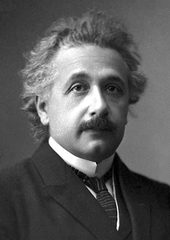
\includegraphics[scale=1]{src/images/lbk-graphics/portraits/einstein-nobel-prize}
\caption*{Einstein's official 1921 portrait after receiving the Nobel Prize in Physics}
\end{figure}
%~ \portrait{1.1}{lbk-graphics/portraits/einstein-nobel-prize}%
%~ {Einstein's official 1921 portrait after receiving\lbk the 
%~ Nobel Prize in Physics}
\begin{small}
\begin{quote}
A hundred times every day I remind myself that my inner and 
outer life are based on the labours of other men, living and 
dead, and that I must exert myself in order to give in the 
same measure as I have received and am still receiving... 
\dm \hfill --Albert Einstein 
\end{quote}

%~ \newpage\thispagestyle{empty}



%~ \newpage
\begin{quote} 
Einstein taught us to regard events as the basic 
data of physics. He showed us the full significance of 
inertial frames and inertial observers. It was he who found 
that every inertial observer has his own privately  valid 
time, and, correspondingly, his  own ``instantaneous 
three-spaces'' consisting of all events $(x,y,z,t)$ with 
fixed time coordinate.\\\hfill--W. Rindler, Ref[4], p.61. 
\end{quote}
\end{small}

\newpage
\section{The general boost in 3-vector  notation}
\index{The general boost ! in 3-vector notation}
% \begin{wrapfigure}{r}{50mm}
\begin{figure}[H]
\begin{center}
\begin{tikzpicture}[>=stealth',scale=.7]
\coordinate (O) at (0,0);
\coordinate (Y) at (0,2) ;%(0,2)
\coordinate (X) at (2,0);%(4,0)
\coordinate (Z) at (-1.25,-1.25) ;% (-2.5,2.5)
%
\draw[thick,->] (O) -- (X) ;
\draw[thick,->] (O) -- (Y) ;
\draw[thick,->] (O) -- (Z) ;
\draw[below] (O)++(.1,0) node{\scriptsize $O$};
\draw[right]  (X) node{\scriptsize $X$};
\draw[above]  (Y) node{\scriptsize $Y$};
\draw[left]  (Z) node{\scriptsize $Z$};
%
\begin{scope}[xshift=3cm,yshift=1.5cm, thick]
\coordinate (O') at (0,0);
\coordinate (2O') at  ($(O)!.5!(O')$);
\coordinate (Y') at (0,2) ;
\coordinate (X') at (2,0);
\coordinate (Z') at (-1.25,-1.25) ;
%
\draw[thick,->] (O') -- (X') ;
\draw[thick,->] (O') -- (Y') ;
\draw[thick,->] (O') -- (Z') ;
\draw[below] (O')++(.1,0) node{\scriptsize $O'$};
\draw[right]  (X') node{\scriptsize $X'$};
\draw[above]  (Y') node{\scriptsize $Y'$};
\draw[right]  (Z') ++(.2,.2)node{\scriptsize $Z'$};
\end{scope}
\draw[thick] (2O') -- (O') ;
\draw[thick,->] (O) --(2O') ;
\draw[above]  (2O') node{\scriptsize $\veca{\gkb}$};
\end{tikzpicture}
\end{center}
\caption{A \textsl{schematic} diagram illustrating the 
general boost: Relative to the frame of reference $S$, 
the 
frame of reference $S'$ moves as a rigid body, 
uniformly, 
without rotation.} \label{fig6.1}
\end{figure}

In 3-vector notation, the {general boost} discussed in 
the
previous chapter is given by
\begin{align}\label{pmadd3}
w'&=\gkg(w-\veca{\gkb}\dotp\veca{r}\, ),\quad
\veca{\gkb}\dotp\veca{r} \equiv \gkb_1 x+\gkb_2 
y+\gkb_3 
z,\\
\pvec{r} & =\veca{r} + \big[-\gkg 
w+(\gkg-1)(\veca{\gkb}\dotp
\veca{r}/\gkb^2) \big] \,\veca{\gkb}, \label{pmadd4}
\end{align}
where  we have split the space and time coordinates of 
a 
general event $P$ in the two frames as $(w,x,y,z)$ 
$\equiv$ 
$(w,\veca{r}\,)$ and $(w' ,x' ,y' ,z' )$ $\equiv 
(w',\pvec{r}\,)$. Note that, here, $w'=ct'$, and $w 
=ct$, 
define the instants of occurrence  and  $\pvec{r}$, 
and 
$\veca{r}$ are the spatial positions  of the event $P$ 
in 
the 
two Lorentz frames.

Also, we should understand Eqn.\eqref{pmadd4} only as  
a 
shorthand\footnote{See Chapter~1 of Hagedorn's book 
Relativistic Kinematics by Hagedorn [4]. Such 3-vector 
equations are also used in Landau and Lifshitz 
[2].} Usually, a vector equation, say $\veca{a}= 
\veca{b}$, is 
a statement of the equality of the corresponding 
components 
of the vectors $\veca{a}$ and  $\veca{b}$ in the 
\textsl{same 
basis}. For example, if $(a_x,a_y,a_z)$ and 
$(b_x,b_y,b_z)$ 
are the components of  $\veca{a}$ and $\veca{b} $ in 
the basis 
$\{\eye,\jay,\kay\}$, then $\veca{a} = \veca{b} 
\Rightarrow 
a_x=b_x $, $ a_y=b_y$ and $a_z=b_z$. On the other 
hand, 
note that we equate components of two vectors in 
\textsl{two 
different bases in Eqn.\eqref{pmadd4} and obtain the 
following set of three 
equations}:
\begin{align}\label{6.3x}
 x'=x-\gkg\gkb_1 w +(\gkg-1)(\veca{\gkb}\dotp
\veca{r})\gkb_1/\gkb^2,\notag\\
 y'=y-\gkg\gkb_2 w +(\gkg-1)(\veca{\gkb}\dotp
\veca{r})\gkb_2/\gkb^2,\\
 z'=z-\gkg\gkb_3 w +(\gkg-1)(\veca{\gkb}\dotp
\veca{r})\gkb_3/\gkb^2.\notag,
\end{align}
where we have written $\gkb_x\equiv\gkb_1$, 
$\gkb_y\equiv\gkb_2$ and $\gkb_z\equiv\gkb_3$.
\begin{quote}
\textit{This notation is rather \textsl{unusual} for a 
vector equation. Here, for example, in 
Eqn.\eqref{6.3x}, the first equation is obtained by 
equating the coefficient of $\,\eye\,'\,$ on the left 
hand side to the coefficient of $\,\eye\,$ on the 
right hand side. The two other equations in 
Eqn.\eqref{6.3x} are obtained similarly. }
\end{quote}

It is  also useful to note the following 
transformation formulae applicable to finite 
coordinate 
differences: If $\tilde{X}_1 \equiv 
(w_1,\veca{r_1}\,) $ and  $\tilde{X}_2 \equiv 
(w_2,\pvec{r_2}\,) $ are the $S$-frame coordinates of 
two 
arbitrary events, then applying the general boost 
equations .\eqref{pmadd3} and \eqref{pmadd4} separately 
to  
$X_1$ and $X_2$ and subtracting the expressions for 
$X'_1$ 
from those of  $X'_1$, we get 
\begin{align}\label{pmadd4a}
&\Delta w'=\gkg(\Delta w-\veca{\gkb}\dotp \Delta 
\veca{r})\,,\\
&\Delta \pvec{r} =\Delta \veca{r} + \big\{-\gkg \Delta 
w 
+(\gkg-1) (\veca{\gkb}\dotp \Delta\veca{r}/\gkb^2) 
\big\}\,\veca{\gkb}\label{pmadd4b}.
\end{align}

\exm Obtain the transformation rule of a contra 
4-vector 
$(A^0,\veca{A})$ under a general boost. 

\soln Since the spacetime coordinates of an  event are 
the 
components of a typical contravariant 4-vector,  we 
may 
replace $(x^0,\veca{r})$ in Eqs.\eqref{pmadd3} and 
\eqref{pmadd4} by $(A^0,\veca{A})$ and obtain the 
following 
transformation rule for a contra 4-vector 
$(A^0,\veca{A})$ 
under a general boost:
\begin{align*}\tag{6.5}
&A^{0'}=\gkg(A^{0}-\veca{\gkb}\dotp\veca{A})\\
&\pvec{A}=\veca{A}+\big[-\gkg A^{0}
+(\gkg-1)(\veca{\gkb}\dotp\veca{A}/\gkb^2)]\veca{\gkb},
\end{align*}\ebx

\vspace{-.3cm}

\section{Transformation of 3-velocity}

Let $\veca{r}=\veca{r}(t)$ be the space-orbit of a 
point 
object 
$ P $ in the Lorentz frame $S$ and 
\begin{align*}
\veca{u} \equiv \dv{\veca{r}}{t} =\eye\dv{x}{t}
+ \jay\dv{y}{t} +  \kay\dv{z}{t},
\end{align*} 
be its 3-velocity in $S$.  In another Lorentz frame 
$S'$ 
related to $S$ by the general boost 
Eqns.\eqref{pmadd3}-\eqref{pmadd4}, the 3-velocity 
$\pvec{u}(t') $ of $P$ is given by
\begin{align*}
\pvec{u} 
&=\dv{\pvec{r}}{t'}=\eye' u'_x +\jay' u'_y 
+\kay'u'_z =\eye' \dv{x'}{t'}+\jay' \dv{y'}{t'} 
+ \kay' \dv{z'}{t'} .
\end{align*}
Now, using Eqn.\eqref{pmadd4b}, taking all the 
coordinate 
differences as the corresponding coordinate 
differentials, 
we get
\begin{align*}
&\dv{\pvec{r}}{w'}=\frac {\dd{\veca{r}}
+\{ (\gkg-1)(\veca{\gkb}\dotp \dd{\veca{r}})/\gkb^2 
\}\, 
\veca{\gkb}-\gkg\veca{\gkb}\,\dd{w}} {\gkg \,\dd{w}
-\gkg \veca{\gkb}\dotp \dd{\veca{r}}} 
\end{align*}
\begin{align*}
= \frac{(\dd \veca{r}/\dd w)+\{ (\gkg-1)(\veca{\gkb} 
\dotp \dd\veca{r}/\dd w)/\gkb^2 \}\, 
\veca{\gkb}-\gkg\veca{\gkb}} {\gkg(1 - \veca{\gkb} 
\dotp \dd\veca{r}/\dd w)}
\end{align*}
which is the same as
\begin{align}\label{pm4}
\pvec{u}=\frac{\veca{u}+ (\gkg-1)
(\veca{\gkb}\dotp\veca{u}/\gkb^2)\veca{\gkb}
-c\gkg\veca{\gkb}}{\gkg
(1-\veca{\gkb}\dotp \veca{u}/c)}.
\end{align}
As remarked earlier, this equation, like 
Eqns.\eqref{pmadd4} 
or \eqref{pmadd4b}, is only a compact way of expressing 
the 
set of three equations a typical one among them being
\begin{align*}
u'_x=\frac{u_x+ (\gkg-1)(\veca{\gkb}\dotp 
\veca{u}/\gkb^2) \gkb_1- c\gkg \gkb_1} 
{\gkg (1-\veca{\gkb}\dotp \veca{u}/c)}\,.
\end{align*}
In the Newtonian limit $c\rightarrow \infty$, 
Eqn.\eqref{pm4} approximates to
\begin{align}\label{pm4-add}
\pvec{u}=\veca{u} -\veca{v},
\end{align}
which is the familiar Galilean velocity composition 
formula.

The more familiar velocity addition (composition) 
formulae 
under an $x$-Lorentz-boost, follow from Eqn.\eqref{pm4} 
as 
a 
special case by setting $\gkb_1 
=\gkb,\;\gkb_2=\gkb_3=0$ in 
it: In an obvious notation, we have
\begin{align*}
(u'_1,u'_2,u'_3)&=\frac{(u_1,u_2,u_3) +u_1 
(\gkg-1)
(1,0,0)-\gkg(v,0,0)}{\gkg [1-vu_1/c^2]}\,,
\end{align*}
which may also be displayed as
\begin{align}\label{pm5}
u'_1&=\frac{u_1 -v}{1-vu_1/c^2},\notag\\ u'_2 &=
\frac{u_2\sqrt{1-v^2/c^2} }{ 1-vu_1/c^2}, \notag\\ 
u'_3&=\frac{u_3\sqrt{1-v^2/c^2} }{1-vu_1/c^2}\,.
\end{align}

\subsection{Transformation of the gamma-factor} 
Let $P$ be a material particle moving with the 
3-velocity  
$\veca{u}=\dd \veca{r}/\dd t$ in a Lorentz frame $S$. 
Let 
$\Gamma\equiv (1-u^2/c^2)^{-1/2}$ be the 'particle 
gamma-factor' associated with $P$. In another  Lorentz 
frame 
$S'$, related to $S$ by a general boost in Eqns. 
\eqref{pmadd3} and \eqref{pmadd4}, let $\veca{u}'=\dd 
\pvec{r}/\dd t'$ be the 3-velocity and   
$\Gamma'\equiv 
(1-{u'}^2/c^2)^{-1/2}$ be the 'gamma-factor' 
associated 
with 
$P$. We now wish to determine the equation connecting  
$\Gamma'$ and $\Gamma$.

Consider two infinitesimally separated events $A$ and 
$B$ on the world line of $P$ with coordinates 
$(ct,\veca{r}$ 
and $(ct+c\dd t,\,  \veca{r}+\dd \veca{r})$ in $S$ and 
$(ct',\veca{r}')$ and $(ct'+c\dd t',\,\veca{r}'\dd 
\veca{r}')$ 
in 
$S$ and $S'$ respectively. Then, we have
\begin{align}\label{6.9x}
 (c\dd t)^2-(\dd \veca{r})^2=(c\dd {t'})^2-(\dd 
\pvec{r})^2
\end{align}
which may be rearranged as
\begin{align}\label{6.10x}
c^2 (\dd t)^2[1-u^2/c^2]=c^2 (\dd t')^2[1-(u')^2/c^2].
\end{align}
This is the same as
\begin{align}\label{6.11x}
c^2  (\dd t)^2/\Gamma^2=c^2 (\dd t')^2/{\Gamma'}^2.
\end{align}
In this, we may replace $c^2(\dd t')^2$ using
Eqn.\eqref{pmadd3} to get
\begin{align}\label{6.12x}
c^2  (\dd t)^2{\Gamma'}^2=\gkg^2\big(c\dd t-\veca{\gkb}
\dotp \dd \veca{r}\big)^2 {\Gamma}^2.
\end{align}
Finally, dividing throughout by $(c\dd t)^2$, taking 
(positive) square-roots, we get
\begin{align}\label{6.13x}
\Gamma'=\big[\gkg\big(1-\veca{\gkb} 
\dotp\veca{u}/c\big)
\big]\Gamma,
\end{align}
which is the required relation between $\Gamma$ and 
$\Gamma'$ of a material particle in the Lorentz frames 
$S$ 
and $S'$ connected by a general boost.

\exm Prove the Lorentz invariance of the photon speed 
using 
Eqn.\eqref{pm4}.
\soln Taking $\veca{u}=c\what{n}$ for a photon 
travelling in 
the direction $\what{n}$, in the Lorentz frame $S$, we 
express Eqn.\eqref{pm4} as
\begin{align}\label{pm6}
\pvec{u}&=c\,\hat{n}', \textsl{ where }\notag\\
\hat{n}' &=\frac{\hat{n}+ \hat{\gkb}\,(\gkg-1)  
(\hat{\gkb}\dotp\hat{n}) -\gkg\veca{\gkb}} 
{\gkg (1-\veca{\gkb}\dotp \hat{n})}\notag\\
&=\frac{\hat{n} +[(\gkg-1) \cos\theta
-\gkg\gkb]\,\hat{\gkb}} {\gkg (1-\gkb\cos\theta)}\,,
\end{align}
and $\theta$ is the angle between $\hat{n}$ and 
$\hat{\gkb}$. The expression $\pvec{u}=c\,\hat{n}'$, 
where $\hat{n}'$ is a unit-3-vector, of the 
velocity of the photon in the Lorentz frame $S'$ 
clearly 
shows that {the photon has the same speed $c$ in all 
Lorentz frames}.\ebx

\exm  In Eqn.\eqref{pm6}, verify that  $\hat{n}'$ is 
indeed 
a unit vector as its notation indicates.
\soln From  Eqn.\eqref{pm6}, we note that
\begin{align*}
&\gkg^2 (1-\gkb\cos\theta)^2 
(\hat{n}'\dotp\hat{n}')\\
&= \hat{n}\dotp\hat{n}+2[(\gkg-1)\hat{n}\dotp 
\hat{\gkb} -\gkg\gkb] (\hat{n}\dotp\hat{\gkb}) 
+[(\gkg-1)\hat{n}\dotp\hat{\gkb} -\gkg\gkb]^2 
(\hat{\gkb}\dotp\hat{\gkb})
\end{align*}

\begin{align*}
&=1+2[(\gkg-1)\cos\theta-\gkg\gkb] \cos\theta 
+[(\gkg-1)\cos\theta -\gkg\gkb]^2\\
&=1+(\gkg^2-1)\cos^2\theta+\gkg^2\gkb^2 -2
\gkg^2 \gkb\cos\theta\\
&=1+\gkg^2\gkb^2+\gkg^2\gkb^2\cos^2\theta-
2 \gkg^2  \gkb\cos\theta \\&=\gkg^2
+\gkg^2\gkb^2\cos^2\theta 
-2 \gkg^2 \gkb\cos\theta=\gkg^2(1-\gkb\cos\theta)^2,
\end{align*}
where we have used the identity $\gkg^2 
=1+\gkg^2\gkb^2$. Thus,  $(\hat{n}' \dotp \hat{n}')$ 
must be equal to $1$ showing that $\hat{n}'$ is indeed 
a 
unit vector. 

\section{Geometrical definition of a\\ Lorentz-frame}
Let $S:\{x^\gkm\}$ be a Lorentz frame. 

\dfn A a one-dimensional subspace of $\textsl{M}$ 
defined 
by the parametric equations 
\begin{align}
K: x^\gkm=x^\gkm(\gkl), \quad \gkl_1\leq\gkl\leq\gkl_2,
\end{align}
where $\gkl$ is a (real) \textsl{parameter}, is called 
a 
\textsl{curve} in $\textsl{M}$. It is convenient to 
choose 
the parameter $\gkl$ to be Lorentz invariant, but 
whenever 
found convenient, we also use parameters which are not 
Lorentz-invariant. The time-coordinate $t$ of a 
Lorentz 
coordinate system $S:\{x^\gkm\}$ is a typical 
non-Lorentz-invariant curve-parameter that is 
frequently 
employed.

An important parametrized curve in $\textsl{M}$ is the 
world-line of a material particle defined by
\begin{align}
 W:x^\gkm=x^\gkm(\gkt), \quad \gkt_1\leq\gkt\leq\gkt_2,
\end{align}
where $\gkt$ is the invariant proper time along $W$. 
Another important class of parametrized curves in 
$\textsl{M}$ are the \textsl{coordinate-curves} of a 
Lorentz coordinate system such as $S:\{x^\gkm\}$. On a 
$x^0$-coordinate curve of $\{x^\gkm\}$, by definition, 
only 
one of the four coordinates, namely, $x^0=ct$, varies 
from 
event to event while the other three coordinates 
$x^1=x$, 
$x^2=y$ and $x^3=z$, remain constants. Similarly, one 
defines  the $x$, $y$ and $z$ coordinate-curves of the 
system $\{x^\gkm\}$ in $\textsl{M}$.

\begin{figure}[H]
\centering
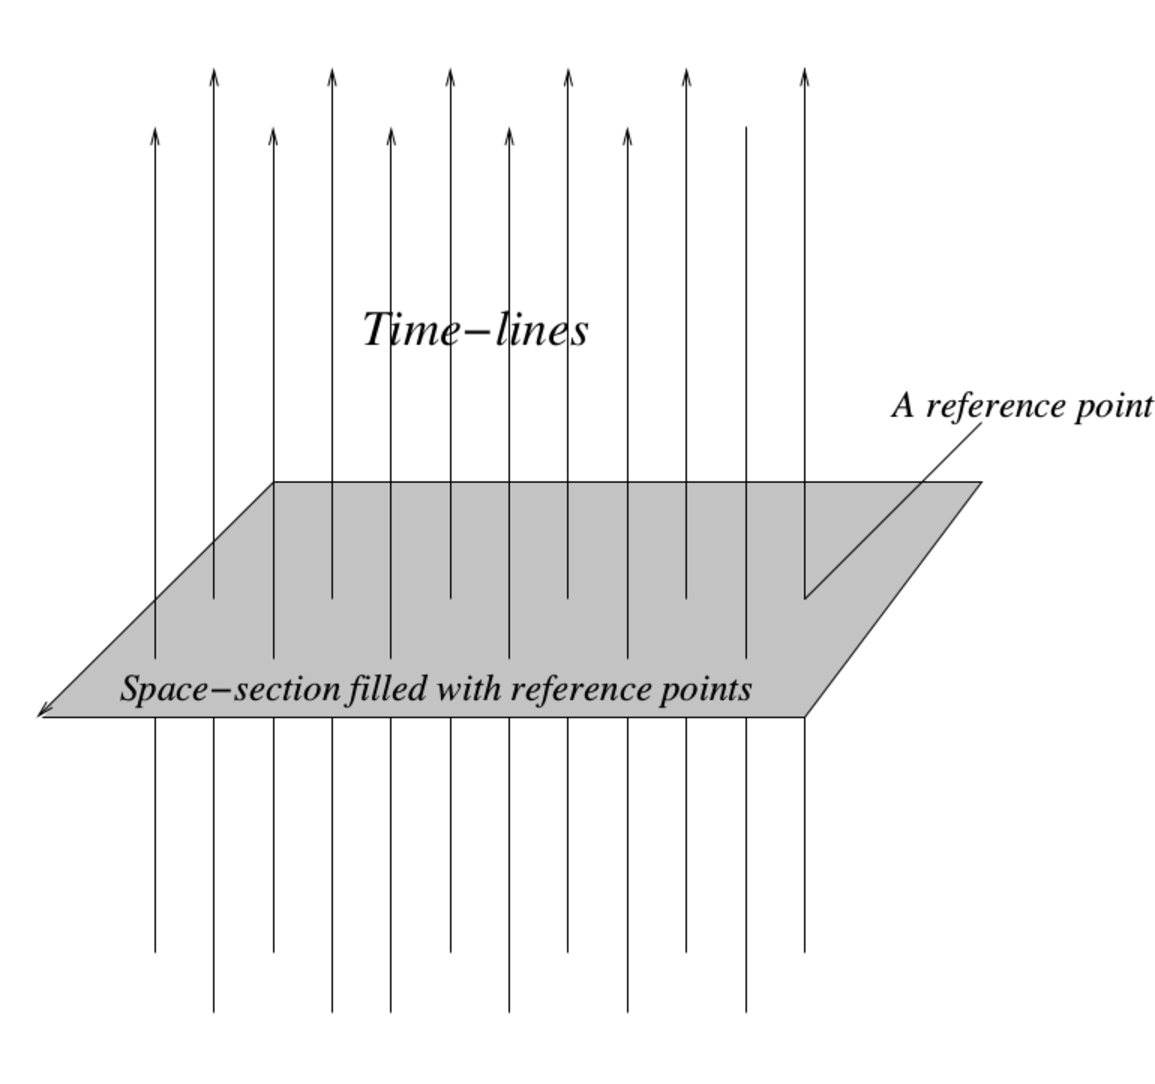
\includegraphics[scale=.3]{src/images/lbk-graphics/space-section-bw}
\caption*{Figure 6.2:~Time-lines of a Lorentz coordinate system}
\end{figure}
%~ \fig{.3}{lbk-graphics/space-section-bw}{Time-lines 
%~ of a Lorentz coordinate system}{fig6.2} 

\newpage
A time-coordinate curve $T$ of $\{x^\gkm\}$ is 
therefore  
described by the equation
\begin{align}\label{T}
T:x=k_1, \quad y=k_2,\quad  z=k_3,
\end{align}
where $k^1, k^2, k^3$, are three fixed real numbers 
which are the $S$-frame coordinates of a spatial point 
$R:(k^1,k^2,k^3)$ in a space-section of $\textsl{M}$ 
orthogonal to $T$. As $(k^1,k^2,k^3)$ are varied 
continuously in the domain 
$-\infty<k^1,k^2,k^3<\infty$, and with precisely one 
time-line corresponding to a fixed spatial point 
$(k^1,k^2,k^3)$, we get a family of time-lines defined 
in Eqn.\eqref{T}) which fill the whole of the 
space-section of $\textsl{M}$ orthogonal to each one of 
the time-lines.
\dfn A space-filling (i.e., 'a space-section filling') 
family of time-lines of a Lorentz (spacetime) 
coordinate 
system $S: \{x^\gkm\}$ is called a  \textsl{congruence} 
of 
time-lines of the Lorentz-frame $S: \{x^\gkm\}$. 

\dfn A time-line $T$ (cf. Eqn.\eqref{T}) of a Lorentz 
coordinate $S: \{x^\gkm\}$ cuts a space-section of 
$\mathbb{M}$, namely   $x^0=$constant, orthogonally in 
a 
space point    $R:(k^1,k^2,k^3)$ called a 
\textsl{reference 
point} of $S:\{x^\gkm\}$.

\dfn The collection $R:\{(k^1,k^2,k^3)\}$ of all 
\textsl{reference-points}  associated with a Lorentz 
coordinate system $S: \{x^\gkm\}$ is called the 
\textsl{frame of reference} provided by it.

\subsection{Motion of  a reference-point of {$S$}{} relative to {$S'$}{}}

By definition, a reference point, say $P$, of the 
Lorentz  
frame $S$ remains permanently at rest relative to $S$. 
In 
other words, the $S$-frame 3-velocity of a reference 
point 
such as $P$ is $\veca{u}=0$. Setting $\veca{u}=0$ in 
the 
velocity transformation formula Eqn.\eqref{pm4}, we get
\begin{align}\label{6.12}
\pvec{u}=-c\veca{\gkb}=-\veca{v},
\end{align}
which is the 3-velocity $\veca{u'}$ of $P$ relative to 
the 
frame $S'$. In other words, a reference point $P$ of 
the 
frame $S'$ moves with a 3-velocity 
$\pvec{u}=-\veca{v}$ 
relative to the frame $S'$. Integrating 
Eqn.\eqref{6.12} 
with respect to $t'$, we get
\begin{align}\label{6.13}
\pvec{r}(t')=-c\veca{\gkb}t'+\veca{\gks},
\end{align}
where $\veca{\gks}$ is a constant (vector) of 
integration. 
This is the $S$-frame equation to the spatial orbit of 
a 
reference point $P$ of the frame $S'$. Now, if we 
recall 
that the $S'$-frame is simply the totality of all its 
reference points which are rigidly fixed relative to 
one 
another, it follows that the $S'$-frame moves with a 
3-velocity $\pvec{u}=-\veca{v}$ relative to the frame 
$S'$.

Normally, without the above demonstration, we  state 
that 
the general boost described in equations \eqref{pmadd3} 
and 
\eqref{pmadd4} represents a transformation between two 
Lorentz  frames $S$ and $S'$ in which, one of the 
frames\footnote{The frame $S$, similarly, would have 
the 
3-velocity $\veca{v'}=c\veca{\gkb'}$ relative to the 
frame 
$S$}, 
say $S'$, moves with the 3-velocity 
$\veca{v}=c\veca{\gkb}$ 
relative to the frame $S$ and also adjoin the 
equations 
\eqref{pmadd3} and \eqref{pmadd4} with the ( schematic! 
) 
diagram in Figure~6.2.  We hope that the above 
discussion 
satisfies  the more serious student.

% Note that the space axes of $S'$, related to  $S'$ 
by 
% the general boost \eqref{str.33} or \eqref{pmadd3}, 
% {always remain parallel} to the corresponding space 
% axes of $S$.

\exm Without using the velocity transformation formula 
Eqn.\eqref{pm4}, directly obtain the equations 
\eqref{6.13} 
 when the two frames $S$ and $S'$ are connected by the 
general boost. 

\soln Let $A=(ct', \pvec{r})=(ct', 0, \gka,0)$ where 
$\gka$ 
is a real constant, be an \textsl{arbitrary} event on 
the 
$y'$-axis of the $S'$-frame. Then, using the inverse 
general boost, namely,
\begin{align}
&w=\gkg[w'+(\veca{\gkb}\dotp \pvec{r})]\notag\\
& x=x'+\gkg\gkb_1 w -(\gkg-1)(\veca{\gkb}\dotp
\pvec{r})\gkb_1/\gkb^2,\notag\\
& y=y'+\gkg\gkb_2 w -(\gkg-1)(\veca{\gkb}\dotp
\pvec{r})\gkb_2/\gkb^2,\\
& z=z'+\gkg\gkb_3 w -(\gkg-1)(\veca{\gkb}\dotp
\pvec{r})\gkb_3/\gkb^2,\notag
\end{align}
we calculate the $S$-frame coordinates of $A$ given 
below: 
\begin{align}\label{6.23}
&ct= \gkg ct'  +\gkg\gkb_2 \gka,\\\label{6.24}
&x_k=\gkg \gkb_k  ct' +[(\gkg-1) \gkb_k 
\gkb_2/\gkb^2]\gka
+\delta_{k2}\gka,\quad k=1,2,3.
\end{align}
Using Eqn.\eqref{6.23}, we  eliminate the term $\gkg 
ct'$ 
from the  equations \eqref{6.24} and obtain, after 
some 
simplification and rearrangement,
\begin{align}\label{6.25}
x_k&=\gkb_k ct- \gks_k,\quad k=1,2,3,
\end{align}
where we have defined the three constants 
\begin{align}\label{6.26}
 \gks_k\equiv  \delta_{k2}
\gka+(\gkg-1)\gka\gkb_2\gkb_k/\gkg\gkb^2.
\end{align}\ebx

\exm Discuss the previous example 6.1, in the special 
case 
of an $x$-boost, for a reference point $A=(ct', 
\pvec{r})  =(ct', 0, \gka,0)$ on the $y'$-axis of the 
$S'$-frame where $\gka$ is an arbitrary real constant.

\soln 
 
\begin{figure}[H]
\begin{center}
\begin{tikzpicture}
% \draw[help lines,step=.25,lightgray] (-4,-4) 
grid(4,4);
%   \foreach \y in {-4,-3.5,...,4}
%     \draw (-4.2,\y) node[left]{\tiny\y} ;
%   \foreach \x in {-4,-3.5,...,5}
%     \draw (\x,-4.2) node[below]{\tiny\x} ;
\node at (0,0)
{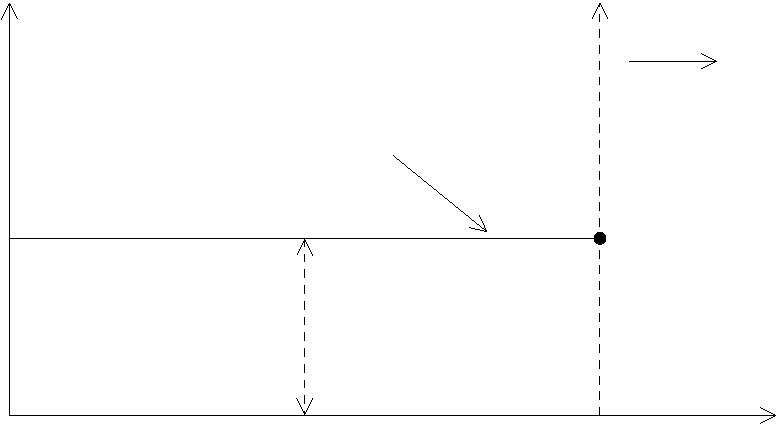
\includegraphics[scale=.4]{src/images/lbk-graphics/1-blank.pdf}};
\node at (2.85,-1.5) {\small  $X$} ;
\node at (-2.5,1.7) {\small  $Y$} ;
\node at (1.55,1.7) {\small  $Y'$} ;
\node at (-2.85,-1.5) {\small  $O$} ;
\node at (1.79, -.2) {\small  $A$} ;
\node at (-1.3,.55) {\small  \text{Trajectory of $A$ in 
the
$S$-frame}} ;
\node at (-.8, -.75) {\small  $ \gka$} ;
\end{tikzpicture}
\caption*{Figure 6.3}\label{fig6.3}
\end{center}
\end{figure}
For an $x$-boost, for which $\gkb_2=\gkb_3=0$ and 
$\gkb_1=\gkb=v/c$, we get, using the equations 
\eqref{6.25} 
and \eqref{6.26},  $\gks_1=\gks_3=0$ and $\gks_2=\gka$ 
so that
\begin{align}
\label{6.27} x_1\equiv x= vt,\; y=\gka,\; z= 0.
\end{align}
This equation shows that $A$ moves as shown in 
Figure~6.4. 
The $S'$ frame reference point  $A:(0, \gka,0)$ (which 
lies 
permanently on the $y'$-axis of the $S'$-frame at $y'= 
\gka$) moves in the $x-y$ plane of $S$ on a straight 
line 
parallel to the $x-$axis (at $y= \gka$, see 
figure~6.4) 
with a uniform velocity $\eye c\gkb=\eye v$. As $\gka$ 
is 
arbitrary, this observation implies that, 'as observed 
from 
$S$, the entire $y'$-axis of the $S'$-frame moves 
parallel 
to the $y$-axis of the $S$-frame with a uniform 
velocity\lbk  $\eye c\gkb=\eye v$'.\ebx

\vspace{-.2cm}

\section{Change in the direction of 
motion}\index{Lorentz 
transformation ! change in the direction 
of motion}
For convenience, we reorient the axes of the frame 
$S:OXYZ$ 
such that the velocity $\veca{u}$ of a material 
particle 
(or, 
photon) under consideration is in the $X-Y$ plane at a 
given moment. Then,
\begin{align*}
\veca{u}=(u\cos\gkq)\eye+ (u\sin\gkq)\jay,
\end{align*}
in  $S$ and
\begin{align*}
\pvec{u}=(u'\cos\gkq')\eye'+ (u'\sin\gkq')\jay',
\end{align*}
in $S'$ by virtue of \eqref{pm5}. (See Figure~6.5.)

\begin{figure}[H]
\centering
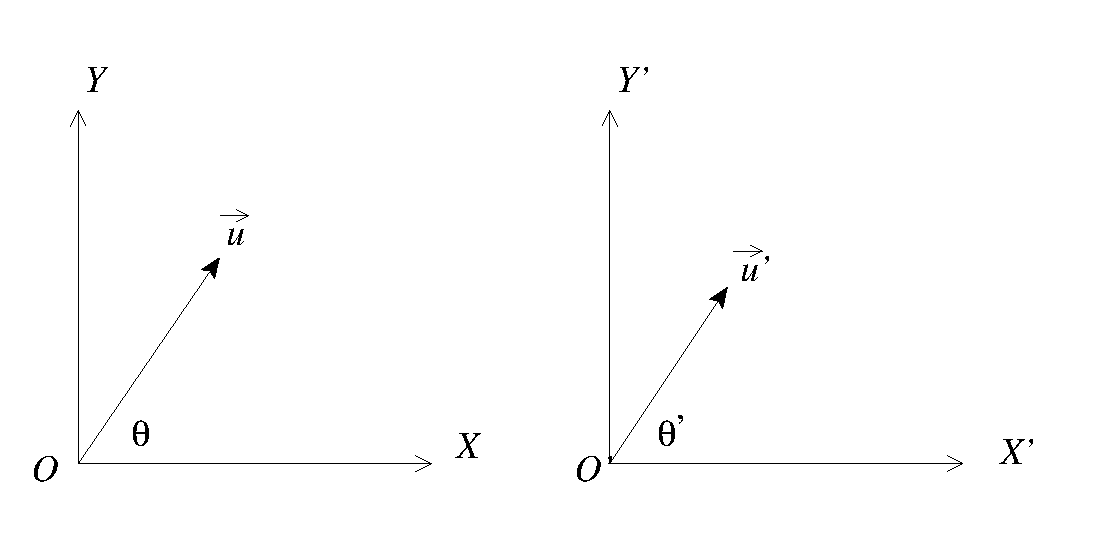
\includegraphics[scale=.4]{src/images/lbk-graphics/aberration}
\caption*{Figure 6.4:~Change in the 
direction of motion}
\end{figure}
%~ \fig{.4}{lbk-graphics/aberration}{Change in the 
%~ direction of motion}{fig6.4}


Dividing $u_y$ by  $u_x$, we get
\begin{align}\label{pm-add-1}
\tan\gkq= \frac{u'_y\sqrt{1-v^2/c^2}}{u'_x+v}=
\frac{u'\sin\gkq'\sqrt{1-v^2/c^2}}{u'\cos\gkq'+v}\,,
\end{align}
which describes the change in the direction of motion of a 
particle, or, a light ray, under an $x$-boost.

\subsection{Aberration of light}
\index{aberration of light}
The position of a star as determined by a telescope has been 
observed to undergo a periodic apparent motion  about its 
real (true) location. This phenomenon is known as the 
\textsl{aberration of light}. It is also referred to as 
astronomical aberration or stellar aberration. Historically, 
aberration of light was discovered and explained  by  James 
Bradley, in 1725. He correctly attributed it to the finite 
speed of light and the motion of Earth in its orbit around 
the Sun.

Setting $u'=c$ in Eqn.\eqref{pm-add-1}, we get the following 
(relativistic) formula describing the aberration of light 
under an $x$-boost:
\begin{align}\label{pm-add-2}
\tan\gkq= 
\frac{(\sin\gkq')\sqrt{1-v^2/c^2}}{(\cos\gkq'+v/c)}\,.
\end{align}

\exm Obtain the Galilean analogue of the aberration 
formula
\eqref{pm-add-2}.
\soln Let us choose a Galilean frame $OXYZ$ at rest in the 
absolute space such that a ray of light from a chosen 
distant star has a velocity $\veca{u} = c(\cos\gkq)eye 
+c(\sin\gkq)\jay$ in it, where $c$ is the speed of light in 
$S$. Further, at a given moment of time, let the velocity of 
the Earth in its orbit around the Sun be $\veca{v}=v\eye$ 
relative to $S$. Then, using the Galilean velocity addition 
formula \eqref{gr.6}, we get
\begin{align}
u_x=(u'_x+v),\quad u_y=u'_y,
\end{align}
where $\pvec{u} = c'(\cos\gkq')\eye +c'(\sin\gkq)\jay\ $ is 
the velocity and $c$ is the speed of the star-light in $S'$ 
so that
\begin{align}\label{pm-galilean}
\tan\gkq=\frac{u_y}{u_x}=\frac{u'_y}{u'_x+v}
=\frac{c'\sin\gkq'}{c'\cos\gkq'+v}
=\frac{\sin\gkq'}{\cos\gkq'+v/c'}.
\end{align}
Equation  \eqref{pm-galilean} is the Galilean analogue 
of 
the relativistic aberration formula  \eqref{pm-add-2}. 
It 
shows that a light ray which travels in the $X-Y$ plane 
of 
$S$ making an angle $\gkq$ with the $X$-axis, moves 
along 
the spatial direction making an angle $\gkq'$ in the 
Galilean frame $S'$. Note that $c'$ above is the speed 
of 
light in the earth-bound frame $S'$ and it hardly 
differs 
from the speed $c$  of light in the absolute frame $S$ 
in 
which ether is supposed to  be at rest. \ebx

\begin{figure}[H]
\begin{center}
\begin{tikzpicture}
%\draw[help lines,step=.25,lightgray] (-4,-4) 
grid(4,4);
%   \foreach \y in {-4,-3.5,...,4}
%     \draw (-4.2,\y) node[left]{\tiny\y} ;
%   \foreach \x in {-4,-3.5,...,5}
%     \draw (\x,-4.2) node[below]{\tiny\x} ;
\node at (0,0)
{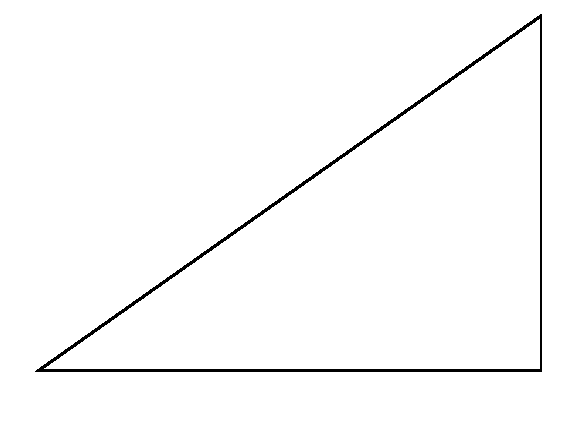
\includegraphics[scale=.4]{src/images/lbk-graphics/triangle.pdf}
};
\node at (.25,-1.4)[left]{\small  $b$} ;
\node at (2.15,0)[left]{\small  $a$} ;
\node at (-.9,-.85)[left]{\small  $\gkq$} ;
\end{tikzpicture}
\end{center}
\caption*{Figure 6.5:}\label{fig6.5}
\end{figure}
Using the basic formula \eqref{pm-add-2}, we now obtain 
 two 
useful approximate expressions for  $\sin\gkq$ and 
$\cos\gkq$: Looking at the right-angled triangle in 
\figref{fig6.5}, where  
$a\equiv\sin\gkq'\sqrt{1-v^2/c^2}$ 
and $b\equiv(\cos\gkq'+v/c)$, we get
\begin{align}\label{pm-add-3}
\sin\gkq&=\frac{\sin\gkq'\sqrt{1-v^2/c^2}}
{\sqrt{(1-v^2/c^2)\sin^2\gkq'+(\cos\gkq'+v/c)^2}}\,,\\
\label{pm-add-4}
\cos\gkq&=\frac{(\cos\gkq'+v/c)}
{\sqrt{(1-v^2/c^2)\sin^2\gkq'+(\cos\gkq'+v/c)^2}}\,,
\end{align}
Now, we observe that
\begin{align*}
&(1-v^2/c^2)\sin^2\gkq'+(\cos\gkq'+v/c)^2 \\
&=(\sin^2\gkq'+\cos^2\gkq')+(v^2/c^2)(1-\sin^2\gkq')
+2(v/c)\cos\gkq'\notag\\
&=1+2(v/c)\cos\gkq'+(v^2/c^2)\cos^2\gkq'= 
\big(1 + (v/c)\cos\gkq'\big)^2,
\end{align*}
so that Eqns.\eqref{pm-add-3} and \eqref{pm-add-4} may 
be 
expressed as
\begin{align}\label{pm-add-5}
&\sin\gkq=\frac{\sin\gkq'\sqrt{1-v^2/c^2}}
{1+(v/c)\cos\gkq'}\,,\\ \label{pm-add-6}
&\cos\gkq=\frac{(\cos\gkq'+v/c)}{1+(v/c)\cos\gkq'}\,.
\end{align}
In the non-relativistic limit of $v<<c$, retaining only 
 
terms of the first order in $v/c$, we may approximate  
 
Eqn.\eqref{pm-add-5} as,
\begin{align*}
 \sin\gkq&\approx(\sin\gkq')
\big(1+\frac{v}{c}\cos\gkq'\big)^{-1}\approx
(\sin\gkq')(1-\frac{v}{c}\cos\gkq')
\end{align*}
so that
\begin{align*}\tag{A}
&\sin\gkq-\sin\gkq'\approx 
-\frac{v}{c}\sin\gkq'\cos\gkq'.\end{align*}
We may rewrite the left hand side of equation (A) as 
\begin{align*}
&2\sin[(\gkq-\gkq')/2]\cos[(\gkq+\gkq')/2]  
\approx2\sin[(\gkq-\gkq')/2]\cos\gkq'.
\end{align*}
Now if we define the 'tilt-angle', or the angle of 
aberration by $\Delta\gkq\equiv \gkq'-\gkq$, we may 
express 
the  relation (A) as
\begin{align*}
-(\Delta\gkq)\cos\gkq'\approx 
-\frac{v}{c}\sin\gkq'\cos\gkq'.
\end{align*}
Finally, cancelling off the term $-\cos\gkq'$ on 
either 
side, we get
\begin{align}
\Delta\gkq\approx \frac{v}{c}\sin\gkq',
\end{align}
which is a useful expression for the 'tilt-angle'  
$\Delta\gkq$. In particular, when $\gkq'=-\pi/2$ which 
corresponds to a light ray coming down 'vertically', we 
get 
$\Delta\gkq\approx -v/c$.

\section{The rest-frame of a material particle}
\index{rest-frame of a material particle}
Consider a material particle which moves in the Lorentz
frame $S$ with the constant 3-velocity $\veca{u} \equiv 
u 
\hat{u}, \quad 0\leqslant u<c$. Let us calculate its 
3-velocity  $\pvec{u}$ in the Lorentz frame $S'$ 
related 
to $S$ by the general boost given by Eqns. 
\eqref{pmadd3}- 
\eqref{pmadd4}. Setting $\veca{\gkb}=\veca{u}/c$ in 
Eqn.\eqref{pm4}, we get\\ 
\vspace*{-1\bsk}\begin{align*} 
\pvec{u}=\frac{\veca{u}+ (\gkg-1) 
(\veca{u}\dotp\veca{u}/u^2)\veca{u}-\gkg\veca{u}}{\gkg 
(1-\veca{u}\dotp \veca{u}/c^2)}=0. 
\end{align*} 
\begin{figure}[ht]
\begin{center}
\begin{tikzpicture}
%   \draw[help lines,step=.25,brown] (-5,-5) grid (5,5) 
;
%   \foreach \y in {-4.5,-4,...,4.5,}
%     \draw (-5.2,\y) node[left]{\small \y} ;
%     \foreach \y in {-5,-4.5,...,4,4.5}
%     \draw (5.2,\y) node[right]{\small \y} ;  
%   \foreach \x in {-4.5,-4,...,5}
%     \draw (\x,5.15) node{\small \x} ;
%       \foreach \x in {-5,-4,...,5}
%     \draw (\x,-5) node[below]{\small \x} ;
\node at (0,0){\includegraphics[scale=1]% 
{src/images/lbk-graphics/inrf2.pdf}};
\node at (-.1,2){\scriptsize $\text{\rm World line of 
the}$}; 
\node at (-.1,1.7){\scriptsize  $\text{\rm material 
particle}$} ;
 \node at (0,1){\small  $ct$} ;
\node at (2.9,-2.25){\small  $y$} ;
\node at (1.5,0.15){\small  $z$} ;
\node at (-.25,-2.25){\small  $x$} ;
\node at (1.5,-1.37){\small  $P$} ;
\end{tikzpicture}
\caption*{Figure 6.6:~Instantaneous rest frame at an event $P$ on 
the 
world line of a material particle}\label{fig6.6}
\end{center}
\end{figure}
Such a frame $S'$ in which the particle has zero 
3-velocity 
is called a \textsl{rest frame of the material 
particle}.

Next,  we consider a material particle which moves with 
a 
{variable} 3-velocity relative to the Lorentz frame 
$S$ 
and define a Lorentz frame\footnote{Given a collection 
of 
material particles (which can be a ``collection'' of 
single 
particle as well) which have a specified motion 
(possibly 
with accelerations) relative to a frame of reference 
$\Sigma$, one can always define a frame $\Sigma'$, 
called a 
{comoving frame} in which the collection of material 
particles is permanently at rest by performing a 
general 
(non-Lorentzian) transformation from $\Sigma$.

Here, we are concerned with Lorentz frames obtained by 
Lorentz transformations only and not with comoving 
frames.}, 
called an \textsl{instantaneous rest frame of the 
material 
particle}, in which the material particle is at rest 
\textsl{at a chosen instant of time} specified in $S$. 
Let 
$\veca{u}(t)$ be the velocity of the particle at the 
instant 
$t$ in $S$. A {general boost} with 
$\veca{\gkb}=\veca{u}(t)/c$, 
transforms from the Lorentz frame $S$ to a new Lorentz 
frame 
${S}^{\bst}_t$ in which the particle is at rest at the 
$S$-frame instant $t$. If the material particle is at 
the 
position $\veca{r}=(x,y,z)$ in the Lorentz frame $S$ at 
the 
$S$-frame instant $t$, then $P :(w=ct,x,y,z)$ is an 
event on 
the world line of the material particle. Therefore,  
${S}^{\bst}_t$ may also be referred to as the 
instantaneous 
rest frame at the event $P$ on the world line of the 
material particle. Thus, we may denote ${S}^{\bst}_t$ 
by the 
more appropriate \footnote{Later, when we discuss the 
timelike tangent 4-vector at an event $P$ to the 
(timelike) 
world line of a material particle, we will observe that 
the 
time-axis of the instantaneous rest frame 
${S}^{\bst}_\sfx{P}$  would be along the timelike 
tangent 
4-vector at the event $P$ to the world line. See 
\figref{fig6.6}.} symbol ${S}^{\bst}_\sfx{P}$.

\hbf{Note} Rest-frames exist only for material 
particles 
and no rest frame, instantaneous or permanent, exists 
for a 
photon.

\section{Relativity of simultaneity}
\index{relativity of simultaneity}
%
%\begin{wrapfigure}[14]{r}{56mm}
\begin {figure}[ht]
\begin{center}
\begin{tikzpicture}[>=stealth',scale=.6]
% \draw[help lines, step=.5,red] (-2,-2) grid (7,7);
% \foreach \x in {-1,0,...,7}\node[left] at (-2,\x)
%{\small \x};
% \foreach \x in {-1,0,...,7}\node[below] at (\x,-2) 
%{\small \x};
\coordinate (A) at (2.5,2);
\coordinate (B) at (2.5,6.5);
\coordinate (C) at (-1,5);
\coordinate (D) at (-1,.5) ;
\coordinate (E) at (.8,3.5) ;
\coordinate (F) at (4.5,3.5) ;
\coordinate (M) at (-.5,2) ;
\coordinate (N) at (2,5) ;
%
\draw[fill=lightgray] (A) -- (B)-- (C)-- (D)-- (A);
\draw[very thick,->] (E) -- (F);
\draw[very thick] (M) -- (N);
\draw[right] (F) node{\scriptsize $\veca{\gkb}$};
\draw[right]  (1.6,1.2) node{\scriptsize 2-flat 
perpendicular to
$\veca{\gkb}$};
\draw[left] (N)++(.2,.2) node{\scriptsize $Q$};
\draw[left] (M)++(.3,.3) node{\scriptsize $P$};
\end{tikzpicture}
\end{center}
\caption*{Figure 6.7:}\label{fig6.7}
 \end{figure}
 
 Two events  $P : x^\gka_\sfx{P}$ and $Q: 
x^\gka_\sfx{Q}$ 
are {simultaneous} in the Lorentz frame $S$ if they 
occur 
at the same time-coordinate in the Lorentz frame $S$. 
Then, $\Delta w_\sfx{PQ}\equiv w_\sfx{Q}-w_\sfx{P}=0$ 
in 
$S$. In another Lorentz frame, say $S'$ related to $S$ 
by 
the general boost Eqns.\eqref{pmadd3}-\eqref{pmadd3}, 
we 
have, from the transformation rule Eqn.\eqref{pmadd4a} 
of 
time-differences,
\begin{align}\label{pm8}
\Delta w'_\sfx{PQ}=\gkg\,\left\{\Delta 
w_\sfx{PQ}-\veca{\gkb}
\dotp\Delta \veca{r}_\sfx{\nnt PQ}\right\},
\end{align}
where, we recall that $\Delta \veca{r}_\sfx{\nnt 
PQ}\equiv 
\veca{r}_\sfx{Q} - \veca{r}_\sfx{P}$. Evidently,  
$\Delta 
w_\sfx{PQ} =0 \nRightarrow \Delta w'_\sfx{PQ} =0$ 
which 
means that two {distinct}\footnote{Two events are 
distinct 
if not all the four coordinates are the same.} events 
which 
are simultaneous relative to $S$ are not simultaneous 
relative to $S'$ {in general}. 

However, a given pair of distinct events which are 
simultaneous relative to $S$ can remain simultaneous 
relative to the Lorentz frame $S'$ if $\veca{\gkb} 
\dotp\Delta  \veca{r}_\sfx{\nnt PQ}=0$. This condition 
implies 
that any two events simultaneous in $S$ and lying on a 
plane 
perpendicular to the unit vector $\hat{n}$, remain 
simultaneous in the Lorentz frame $S'$  obtained from 
$S$ 
by performing the general boost with  $\veca{\gkb}= 
\gkb\, 
\hat{n}$, where  $0\leqslant\gkb <1$.

Since, in general, the simultaneity of two 
\textsl(distinct) 
events is not preserved under a Lorentz transformation, 
we 
say that  \textsl{simultaneity is relative}. This idea 
is 
also conveyed by the statement ``{special relativity 
abolishes the Newtonian notion of absolute 
simultaneity}''.

\section{Time-ordering of events}

Let the event pair $\{P,Q \}$  be separated by the 
displacement  4-vector $(\Delta x_\sfx{PQ})^\gka 
\equiv 
x_\sfx{Q}^\gka-x_\sfx{P}^\gka$.  Then, 
\dfn the two events $P$ and $Q$ are said to be 
\begin{align}\label{pmx9}
\begin{cases}\text{timelike-separated} \\
\text{null-separated} \\
\text{spacelike-separated},\end{cases}
\text{if} \quad \begin{cases}
|\Delta w_\sfx{PQ}| >  |\Delta  \veca{r}_\sfx{\nnt 
PQ}|\\
|\Delta w_\sfx{PQ}| = |\Delta  \veca{r}_\sfx{\nnt 
PQ}|\\
|\Delta w_\sfx{PQ}|< |\Delta  \veca{r}_\sfx{\nnt PQ}|.
\end{cases}
\end{align}
Thus, for timelike-separated and null-separated 
event-pairs, 
the quantity $(1-\veca{\gkb}\dotp\Delta 
\veca{r}_\sfx{\nnt 
PQ} 
/\Delta w_\sfx{PQ})$ is always \textsl{positive}.  
Then, 
from Eqn.\eqref{pm8} rewritten as
\begin{align}\label{pmx10}
 \Delta w'_\sfx{\nnt PQ}=\gkg\,\Delta w_\sfx{\nnt PQ}
\left\{1-\veca{\gkb}
\dotp\Delta  \veca{r}_\sfx{\nnt PQ}/\Delta w_\sfx{\nnt 
PQ}\right\},
\end{align}
we see that $\Delta w_\sfx{PQ}$ and  $\Delta 
w'_\sfx{PQ}$ 
{are of the same sign for  timelike-separated and 
null-separated event-pairs}\footnote{However, 
Eqn.\eqref{pm8}, in general, does not imply that 
$\Delta 
w_\sfx{PQ}=0 \Rightarrow \Delta w'_\sfx{PQ}=0$.}. In  
other 
words, if $P$ occurs before/after $Q$ in $S$, then $P$ 
occurs before/after $Q$ in $S'$ also. In otherwords,
\begin{quote}
the  \textsl{time-ordering of timelike-separated and  
null-separated event-pairs is absolute}.
\end{quote}
However,  since $|\Delta \veca{r}_\sfx{PQ}|>|\Delta 
w_\sfx{PQ}|$ for all space-like-separated event pairs 
$\{P,Q\}$, the ratio $\veca{\gkb} \dotp\Delta  
\veca{r}_\sfx{\nnt PQ}/\Delta w_\sfx{\nnt PQ}$  can be 
$\gtreqqless 1$, depending on the spacelike-separated  
pair 
$\{P,Q\}$ chosen. Thus, for a chosen 
spacelike-separated  
pair $\{P,Q\}$, $\Delta w'_\sfx{PQ}$ can be greater 
than, 
equal to, or less than   $\Delta w_\sfx{PQ}$. This 
implies 
that  
\begin{quote}
the time-orderng of a pair of spacelike-separated 
events is 
not absolute, but is relative (i.e., frame-dependent).
\end{quote}

\section{Time dilation}
Consider an \textsl{ideal clock} (also called a 
\textsl{standard clock}) $K$ which moves with a 
velocity 
$\veca{v}$ in the Lorentz frame $S$. {We may refer to  
$K$ as 
a  `moving clock' in $S$}. Let $(w,x,y,z)$ be the 
$S$-frame 
coordinates of an event $P$ on the world line of $K$. 
Consider  an event $Q: (w+\dd{w}, x+dx, y+dy, z+dz)$ 
which 
is \textsl{infinitesimally separated} from $P$. 
Introduce 
the instantaneous rest frame  $S'_\sfx{P}$  of the 
clock 
$K$. Then, let $(w',\veca{0})$ and $(w'+\dd{w}', 
\veca{0})$ be 
the $S'_\sfx{P}$-frame coordinates of the same two 
events 
$P$ and $Q$. (Note that  $P$ and $Q$ are at 
rest\footnote{More specifically, we assume that the 
event 
$Q$, which is infinitesimally separated from $P$,  lies 
on 
the 4-tangent to the world line of $K$ at $P$.} in the 
instantaneous rest frame $S'_\sfx{P}$ and occur at the 
same 
space point which we have chosen as the origin 
$\veca{0}$ of 
$S'_\sfx{P}$.) {The time-separation} $d\tau\equiv 
\dd{w}'/c 
$ between $P$ and $Q$ on the world line of the clock 
$K$,  
\textsl{in the instantaneous rest frame of the 
clock}$S'_\sfx{P}$,  is called the \textsl{proper 
time-element} separating $P$ from $Q$. Using the 
Lorentz 
invariance of the (squared) spacetime interval between 
$P$ 
and $Q$, we have
\begin{align*}
 ds^2_\sfx{PQ}&=(\dd{w}')^2=c^2d\tau^2=(\dd{w})^2 -
 (dx^2+dy^2+dz^2) \notag\\&=  c^2dt^2(1-v^2/c^2),
\end{align*}
from which we get the relation
\begin{align}\label{pm9}
 \gkg d\tau=dt.
\end{align}
Here, we  have chosen the 
positive root here assuming that $\tau(t)$ increases 
with 
$t$ along the world line of $K$. Equation \eqref{pm9} 
is  
the \textsl{Larmor-Einstein time-dilation 
formula}. This derivation of the time-dilation 
formula, 
known for its characteristic brevity, is taken from 
the book of Landau and Lifshitz [4]. We urge the 
reader 
to see also the appendix~6B to this chapter in which 
we 
present a more detailed discussion of  time-dilation 
under 
the context of the general time-interval 
transformation 
formula.
\begin{quote}
Clearly, the time-dilation formula implies $d\tau < dt$ 
as 
$\gkg >1$, and this means that the clock $K$, which, 
as 
already mentioned, is a moving clock in $S$, goes slow 
compared to the system of synchronised coordinate 
clocks of 
the Lorentz $S$. One says cryptically, 
`\textsl{moving clocks go slow}''. 
\end{quote}

\index{length contraction}
\section{Length contraction}
\hbf{The length of a rod in a given Lorentz frame} 
Consider a `'rigid rod'' $AB$ 
which moves uniformly with a velocity $\veca{v}$ in 
the 
Lorentz frame $S$. Strictly speaking there are no 
rigid 
bodies according to special relativity.  In this 
context, we 
may quote 
the following passage from Synge's book [1], p.36:
\begin{quote}
``... rigid bodies do not exist in nature--every 
solid is deformed by stress. The Newtonian rigid body 
is 
an idealisation; it may be regarded as the limit of a 
sequence of bodies which are more and more resistant 
to 
deformation. In view of the fact that the speed of 
sound 
in a solid increases with its resistance to 
deformation, we 
must admit that in the Newtonian rigid body the speed 
of 
sound is infinite. There is no objection to such an 
infinite speed in Newtonian theory, but in relativity 
theory the speed of sound is an upper bound which 
cannot be 
exceeded by any signal. Therefore it is useless to seek 
a 
relativistic definition of a rigid body.''  
\end{quote}

%~ \newpage

\begin{figure}[H]
 \begin{center}
\begin{tikzpicture}[>=stealth',scale=.7]
% \draw[help lines, step=.5,red] (0,0) grid (7,7) ;
% \foreach \x in {0,1,...,7}\node[left] at (0,\x) 
% {\small \x} ;
% \foreach \x in {0,1,...,7}\node[below] at (\x,0) 
% {\small \x} ;
%
\coordinate (a) at (2.5,2.5);
\coordinate (b) at (5.5,6) ;
\coordinate (c) at (1,6) ;
\coordinate (a2b) at ( $(a)!.6!(b) $);
\coordinate (a2c) at ( $(a)!.6!(c) $);
\coordinate (b2c) at ( $(b)!.4!(c) $);
\draw[thick] (a) -- (b);
\draw[thick,->] (a) -- (a2b);
\draw[thick] (a) -- (c);
\draw[thick,->] (a) -- (a2c);
\draw[thick] (c) -- (b);
\draw[below] (a) node{\small $O$};
\draw[above] (3.3,6) node{\scriptsize $L 
=|\veca{r}_\sfx{2}(t) -\veca{r}_\sfx{1}(t)|$};
\draw[left] (1,6) node{\small $A$};
\draw[right] (5.5,6) node{\small $B$};
\draw[left] (1.8,4) node{\small $\veca{r}_\sfx{1}(t)$};
\draw[right] (4,4) node{\small $\veca{r}_\sfx{2}(t)$};
\end{tikzpicture}
\caption*{Figure 6.8:~Length of a moving rod}\label{fig6.8}
\end{center}
\end{figure}

However, one may certainly consider bodies which are 
\textsl{sufficiently rigid} for a stated purpose. One 
defines the length $L$ of such a `rigid'  moving rod 
$AB$ in 
$S$ without interfering with its motion\footnote{J. L. 
Synge 
Ref. [1], p.117} as follows: If $\veca{r}_\sfx{1}(t) = 
(x_\sfx{1},y_\sfx{1},z_\sfx{1})$ and 
$\veca{r}_\sfx{2}(t)= 
(x_\sfx{2},y_\sfx{2}, z_\sfx{2})$ are the position 
vectors 
of the two ends of the moving rod at the \textsl{same 
instant} $t$ in $S$, then the length of the (moving) 
rod in 
$S$ is given by
\begin{align*}
L =|\Delta\veca{r}_\sfx{\nnt 12} | = 
|\veca{r}_\sfx{2}(t) -
\veca{r}_\sfx{1}(t)|.
\end{align*}

One may also define, geometrically, the length of a 
moving 
rod as follows: If $W_1$ and $W_2$ denote the world 
lines 
of the two ends of the rod in the Minkowski spacetime, 
then, 
we may restate this definition of the length $L$ of a 
moving 
rod in a given Lorentz frame also as follows : (See 
the 
Example~6.7, especially \figref{fig6.10}.)

\dfn  The length $L$ of a rod relative to a Lorentz 
frame 
$S$ is the spatial distance between any event 
$P:(ct,x_\sfx{1},y_\sfx{1},z_\sfx{1})$ on $W_1$ and 
the 
event $Q:(ct, x_\sfx{2},y_\sfx{2},z_\sfx{2})$ on $W_2$ 
which is \textbf{simultaneous} with the chosen event 
$P$ in 
$S$. 

\hbf{The proper length of a rod} 
Let the rod be at rest in the frame $S'$ which is 
related to 
the frame $S$ mentioned above by an $x$-boost. Then, 
in 
$S'$, the two ends of the rod trace out two world 
lines 
$W_1$ and $W_2$ (see Figure~6.10). On $W_1$, all events 
have 
the \textbf{constant} space coordinates, say,  
$x'_1=a,y'_1=0,z_1'=0$, and only $t'$ varies from event 
to 
event.  Similarly, on $W_2$, all events have the  
\textbf{constant} space coordinates, say, $x'_2=a+L_0, 
y'=0,z'=0$ and only $t'$ varies from event to 
event.\footnote{World lines such as $W_1$ and $W_2$ on 
which the space coordinates $x^{i'}$ (of $S'$) are 
constants and only the time-coordinate $x^{0'}$ (of 
$S'$) varies from event to event, are called 
\textsl{time-coordinate curves of the Lorentz frame 
$S'$}}. 
The spatial-distance in $S'$ between an arbitrary event 
on 
$W_1$ and \textsl{any} event on $W_2$ i.e., 
\begin{align*}
\sqrt{(x'_2-x'_1)^2+(y'_2-y'_1)^2+(z'_2-z'_1)^2}=L_0, 
\end{align*}
gives the length of the rod in $S'$ (which happens to 
be its 
rest-frame) and $L_0$ is called  the \textsl{proper 
length 
of the rod}.  (With reference to the 
Figure~\figref{fig6.9}, 
we may note that the spatial-distances between the 
event 
pairs $A$ and $B$, $A$ and  $D$,  $C$ and $B$, $C$ and 
$D$ 
are all equal to the proper length $L_0$ of the rod.)
\begin{figure}[H]
\begin{center}
\begin{tikzpicture}[>=stealth',scale=.4]
% \draw[help lines, step=.5,red] (-7,-7) grid (8,7) ;
% \foreach \x in {-7,-6,...,7}\node[left] at 
% (-7,\x){\tiny
% \x} ;
% \foreach \x in {-7,-6,...,7,8}\node[below] at (\x,8) 
% {\tiny \x};
\coordinate (O) at (0,0);
\coordinate (X) at (8,0);
%
\draw[thick,gray,->] (O) -- (X) ;
\draw[thick,gray,->] (0,-4) -- (0,4) ;
\draw[left] (O) node{\scriptsize $O$};
\draw[above]  (0,4) node{\small $ct'$};
\draw[right]  (X) node{\scriptsize $X'$};
\draw[thick] (2,4) -- (2,-4) ;
\draw[thick] (5,4) -- (5,-4) ;
\draw[above]  (2,4) node{\scriptsize{$W_1$}};
\draw[above] (5,4) node{\scriptsize{$W_2$}};
\draw[left]  (2,3) node{\scriptsize $A$};
\draw[fill=gray] (2,3) circle (3pt);
\draw [right](5,2.5) node{\scriptsize $B$};
\draw[fill=gray] (5,2.5) circle (3pt);
\draw[left]  (2,-3) node{\scriptsize $C$};
\draw[fill=gray] (2,-3) circle (3pt);
\draw [right](5,-2) node{\scriptsize $D$};
\draw[fill=gray] (5,-2) circle (3pt);
\end{tikzpicture}
\end{center}
\caption*{Figure 6.9:~The proper length of a rod}\label{fig6.9}
\end{figure}

\hbf{Relation between relative and proper lengths} 
Assume 
that the rest-frame $S'$ of the rod is related to the 
Lorentz $S$ by an $x$-boost with $\veca{\gkb}= 
(v/c)\eye$. 
Let $P$ and $Q$ be two events, which are simultaneous 
in 
$S$\footnote{Note that $P$ and $Q$ which are 
simultaneous in 
$S$, would not, in general, be simultaneous in  $S'$ 
(unless 
$\Delta \veca{r}_\sfx{\nnt PQ}\dotp \veca{\gkb}\neq 0 
$).}, 
and occur on the world lines $W_1$ and $W_2$ of the two 
ends 
of the rod. Define the following coordinate differences 
of 
the two events $P$ and $Q$ in $S$:
\begin{align}\label{pmx13}
 \Delta w_\sfx{PQ}&= w_\sfx{Q}(t) - w_\sfx{P}(t) = ct -
 ct=0,\\    \label{pmx14}
 \Delta \veca{r}_\sfx{\nnt PQ}& = 
\veca{r}_\sfx{Q}-\veca{r}_\sfx{P} =L\,\eye,
\end{align}
These coordinate-differences transform to the 
corresponding 
new-differences in $S'$  given below: (cf. 
Eqns.\eqref{pmadd4a} and
\eqref{pmadd4b})
\begin{align}\label{pmx15}
&\Delta w'_\sfx{PQ} \:=\gkg\{\Delta w_\sfx{PQ} -
\veca{\gkb}\dotp\Delta \veca{r}_\sfx{\nnt PQ}\}=-\gkg 
vL/c,\\ &\Delta  \pvec{r}_\sfx{PQ} =\Delta  
\veca{r}_\sfx{\nnt PQ} 
+ \{-\gkg \gkb \Delta w_\sfx{PQ} 
+(\gkg-1)(\hat{\gkb}\dotp \Delta \veca{r}_\sfx{\nnt 
PQ}\,) 
\} \,\hat{\gkb} \notag\\
&\qquad\quad\:= L\, \eye+(\gkg-1)L\eye=\gkg L\,\eye.   
\label{pmx16}
\end{align}
Now, as explained while defining the proper length,  
$|\Delta\pvec{r}_\sfx{PQ}|$ must be the proper length 
$L_0$ of the rod. Thus, from Eqn.\eqref{pmx16} above, 
we get
\begin{align}\label{pmadd14}
 L_0=\gkg L,
\end{align}
which is the \textsl{Lorentz-Fitzgerald length 
contraction  
formula}. Again, as $\gkg >1$, this equation says that 
$L=L_0/\gkg < L_0$. 

\begin{quote}
In other words, the proper length $L_0$ of a rod is 
always 
greater than the length $L$ of the rod determined in a 
Lorentz frame in which the rod is in motion.
\end{quote}
\exm Consider the $x$-boost relating 
two Lorentx frames $S$ 
and $S'$ and a rod at rest on the $x$-axis of the 
frame 
$S$. Draw a spacetime diagram showing the $ct,x$ and 
the 
$ct',x'$ axes of the two frames, the light cone, the 
two 
world lines $W_1$ and $W_2$ of the moving rod and mark 
off 
the proper and relative lengths of the rod in the 
diagram.
\soln 
\begin{figure}[h]
\begin{center}
\begin{tikzpicture}[>=stealth',scale=.4]
% \draw[help lines, step=.5,red] (-7,-7) grid (8,7) ;
% \foreach \x in {-7,-6,...,7}\node[left] at 
% (-7,\x){\tiny 
% \x} ;
% \foreach \x in {-7,-6,...,7,8}\node[below] at (\x,8) 
% {\tiny \x};
\coordinate (O) at (0,0);
\coordinate (X) at (8,0);
\coordinate (X') at (8,4);
\coordinate (L) at (7,7);
\coordinate (Z) at (4,7);
%
\draw[dashed, ->] (O) -- (X) ;
\draw[gray,->] (O) -- (X') ;
\draw[dashed] (O) -- (L) ;
\draw[->] (O) -- (Z) ;
\draw[dashed,->] (0,0) -- (0,7) ;
\draw[very thick] (2,0) -- (5,0) ;
\draw[left] (O) node{\scriptsize $O$};
\draw[above]  (Z) node{\small $ct'$};
\draw[above]  (0,7) node{\small $ct$};
\draw[right]  (X') node{\scriptsize $x'$};
\draw[right]  (X) node{\scriptsize $x$};
\draw[thick] (2,6) -- (2,-2) ;
\draw[thick] (5,6) -- (5,-2) ;
\draw[below]  (2,-2) node{\scriptsize{$W_1$}};
\draw[below] (5,-2) node{\scriptsize{$W_2$}};
\draw[right]  (1.9,.9) node{\scriptsize $A'$};
\draw[fill=gray] (2,1) circle (3pt);
\draw [right](4.9,2.4) node{\scriptsize $B'$};
\draw[fill=gray] (5,2.5) circle (3pt);
\draw[right]  (1.9,-.4) node{\scriptsize $A$};
\draw[fill=gray] (2,0) circle (3pt);
\draw [right](4.9,-.4) node{\scriptsize $B$};
\draw[fill=gray] (5,0) circle (3pt);
\draw[right]  (6,5.9) node{\scriptsize{Light cone}};
\end{tikzpicture}
\end{center}
\caption*{Figure 6.10:~The spacetime diagram for 
Example~6.7}\label{fig6.10}
\end{figure}

In Fig.\figref{fig6.10}, $AB$ and $A'B'$ mark the 
proper 
length and the relative lengths, respectively.
\ebx

\section{Proper-time parametrization}
On the world line $\gks$ of a material particle, mark 
some 
(arbitrary) event as $P_\sfx{0}$. Then, integrating 
Eqn.\eqref{pm9} (on $\gks$ in a Lorentz frame $S$) 
from 
$P_\sfx{0}$ to some other event $P$, which occurs at a 
later 
time $t > t_\sfx{0}$ where  $t_\sfx{0}$ is the 
time-coordinate of $P$, we get
\begin{align}\label{pmadd15a}
 \tau(P)- \tau(P_\sfx{0}) &=
 \pathint{\gks}_\sfx{\hsn P_\sfx{0}}^\sfx{P} \dd \tau
 =\pathint{\gks}_\sfx{\hsn P_\sfx{0}}^\sfx{P} 
\frac{\dd \tau}{\dd t}\,\dd t
=\pathint{\gks}_\sfx{\hsn 
P_\sfx{0}}^\sfx{P}\frac{1}{\Gamma(t)}\,\dd t,
\end{align}
where we have introduced the `\textsl{capital-gamma 
factor}' 
\begin{align}\label{pmadd16a}
\Gamma(t)=\frac{1}{\sqrt{1-u^2/c^2}}.
\end{align}
We may call this `\textsl{the  particle velocity gamma 
factor}' $\Gamma$ to distinguish it from the more 
familiar 
inter-frame gamma factor $\gkg=(1-v^2/c^2)^{-1/2}$ 
(lower case  gamma)  used in Eqn.\eqref{pm9}. Using 
Eqn.\eqref{pmadd15a},  we assign a unique parametric 
value 
$\tau $ to every event on the world line of the 
material 
particle and thus express the equation to the world 
line of 
the material particle in the form
\begin{align}\label{pmadd16}
x^\gka=x^\gka(\tau) ,\quad \tau_1\leq \tau\leq\tau_2,
\end{align}
called the \textsl{proper-time parametric equation} to 
the 
world line of the material particle. We may note that 
one 
cannot define a  proper-time along the world line of a 
photon ({why?}) and one has to use some other 
parameter 
(such as the non-invariant \textsl{coordinate-time} 
parameter $t$) in that case.

\section{4-velocity}
The {4-vector tangent} to the world line of a material 
particle (of rest-mass $m_0$) is given by
\begin{align}\label{pmadd17}
U^\gka=dx^\gka/d\tau=\Gamma\left( c, \dot{x}, \dot{y},
\dot{z}, \right)
=\Gamma\left( c, \veca{u}\right),
\end{align}
where we have used the relation
\begin{align}\label{pmadd17a}
 \Gamma d\tau =dt,
\end{align}
and the \textsl{dot denotes differentiation with 
respect to 
$t$}, is called the (contravariant) {4-velocity} of 
$P$. 
The contravariant 4-vector nature of $U^\gka$ follows 
from 
the fact that $dx^\gka$ is a contravariant 4-vector 
and 
$d\tau$ is a 4-scalar.  Further, {$U^\gka$ is a 
timelike 
4-vector} because
\begin{align*}
U^\gka U_ \gka &=\Gamma^2(c,\veca{u})(c,-\veca{u})
=\Gamma^2(c^2
-\veca{u}\dotp\veca{u})\\&=\Gamma^2(c^2 -u^2)=c^2>0.
\end{align*}
In the instantaneous rest frame $S^{\bst}_t$ of the 
particle, we have $\svec{u}=0$ and $\Gamma^\bst=1$ at 
the 
chosen instant $t$ in $S$,  and as such,
\begin{align}\label{pmadd18}
U^{\bst\, \gka} =( c, \veca{0}),
\end{align}
at the instant $t$ in $S$, or, equivalently, at a 
corresponding instant $t^{\bst}$ in $S^{\bst}$. Then,
\begin{align}\label{pmadd19}
U^\gka( t)U_ \gka( t) =U^{\bst\, \gka}(t)
U^\bst_ \gka(t)=(c,\veca{0})\dotp
(c, \veca{0})=c^2.
\end{align}

\exm Obtain the general 3-velocity addition formula 
Eqn.\eqref{pm4} by applying the transformation rule 
Eqn.(6.1) of a contravariant vector, to the 4-velocity 
$U^\gka$. 

\soln If we set (see \eqref{pmadd17}) $A^0=\Gamma c$ 
and 
$\veca{A}=\Gamma \veca{u}$ in Eqn.(6.1), we get 
\begin{align*}
 &\Gamma' \pvec{u}= \Gamma\veca{u}+\Gamma\big[-\gkg c
+(\gkg-1)(\veca{\gkb}\dotp 
\veca{u}/\gkb^2)\big]\veca{\gkb}.
\end{align*}
Now, we may eliminate $\Gamma/\Gamma'$ from the above 
equation using the transformation formula  
Eqn.\eqref{6.13x} 
for the gamma-factor  and obtain
\begin{align*}
\pvec{u}= \frac{\veca{u}-c\gkg \veca{\gkb}
+(\gkg-1)(\veca{\gkb}\dotp
\veca{u}/\gkb^2)\veca{\gkb}}{\gkg\big(1-\veca{\gkb}
\dotp\veca{u}/c\big) },
\end{align*}
which is Eqn.\eqref{pm4}. \ebx

\subsection{Relative speed between two  material\\ 
particles}
In a Lorentz frame $S$, consider two material 
particles 
$A$ and  $B$ which move with the 3-velocities 
$\veca{u}_\sfx{A}(t)$ and $\veca{u}_\sfx{B}(t)$. We 
wish to 
determine the 3-speed $u^\bst_\sfx{R}(t)$ of $B$ 
relative to 
$A$ (which is the same as that  of $A$ relative to $B$) 
 at 
a given instant of time $t$ in $S$.

Transforming $\veca{u}_\sfx{A}(t)$ to the instantaneous 
rest 
frame $S^\bst_t$ of particle $A$, we get 
$\svec{u}_\sfx{A}(t) =\veca{0}$. Similarly, 
transforming 
$\veca{u}_\sfx{B}(t)$ to $S^\bst_t$ we get 
$\svec{u}_\sfx{B}$ 
which is is the required 3-velocity of $B$ relative to 
$A$. 
Now observe that the 4-velocities of $A$ and $B$ in 
$S^\bst_t$, at the $S$-frame instant $t$, are given by 
$A^{\bst\,\gka}= (c,\veca{0})$ and $B^{\bst\,\gka} =  
\Gamma^\bst_{B}(c,\svec{u}_\sfx{B}(t) )$ so that their 
(invariant) 4-scalar product is given by
\begin{align*}
{A}^\gka {B}_ \gka =A^{\bst\,\gka}  B^\bst_ \gka=c^2
\Gamma^\bst_{B}
=\frac{c^2}{\sqrt{1-{u_\sfx{B}^{\bst\,2}/c^2}}},
\end{align*}
from which we may obtain the 3-speed  $u_\sfx{B}^\bst$ 
of 
particle $B$ with respect to particle $A$. Since the 
relative 3-speeds are equal, we may use a common 
notation 
for them, say, ${u_ \sfx{B}^\bst}= {u_\sfx{A} ^\bst} 
={u_\sfx{R}^\bst}$, and write a formula for 
$u_\sfx{R}^\bst$:
\begin{align}
c^2\Gamma^\bst_\sfx{R}=\frac{c^2}
{\sqrt{1-{u_\sfx{R}^{\bst\, 2} /c^2}}} = A^\gka B_ 
\gka.
\end{align}

\hbf{Note} Incidentally, this formula gives the 
\textsl{kinematical meaning of the Minkowski product of 
two 
timelike  4-vectors} $A^\gka$ and $B^\gka$: The 
Minkowski 
product $A^\gka B_ \gka$ is equal to $c^2$ times the 
the 
gamma-factor $\Gamma^\bst_\sfx{R}$ constructed from 
the 
relative 3-speed $u_\sfx{R}^\bst$ of two timelike 
observers 
(i.e., material particles) whose 4-velocities are 
$A^\gka$ 
and $B^\gka$.

\exm  In a Lorentz frame $S$, two electrons move in 
opposite directions on the $x$-axis with equal uniform 
speeds $u= (\sqrt{3}/2)c $. Find their relative speed.

\soln The 4-velocities of the two electrons in $S$ are\break 
$2(c,u,0,0) $ and $2(c,-u,0, 0) $ whose 4-scalar 
product 
is  $4(c^2+u^2)= 4c^2 (1+u^2/c^2)=4c^2(1+3/4)=7c^2$. 
This must equal $ c^2 \Gamma^\bst_\sfx{R}$ so that 
$(\Gamma^\bst_\sfx{R})^2 = 
((1-\ustar{u}_\sfx{R})^2/c^2)^{-1}  = 49$ which gives 
$\ustar{u}_\sfx{R} =\sqrt{48/49}\,c$. In special 
relativity, 
two speeds $(\sqrt{3}/2)c$ and $(\sqrt{3}/2)c$ in 
opposite 
directions {do not add up to} $2(\sqrt{3}/2)c >c$ as 
in 
Newtonian (Galilean) mechanics, but add up to a speed 
which 
is always less than $c$.  \ebx

\section{4-acceleration of a material particle}
The 4-vector
\begin{align}\label{pmadd20}
A^\gka=\frac{dU^\gka}{d\tau}=\Gamma \frac{d}{dt}(
c\Gamma,\Gamma \veca{u})=\Gamma (
c\dot{\Gamma},\;\dot{\Gamma} \veca{u}+\Gamma\veca{a}),
\end{align}
is called the \textsl{4-acceleration of the material 
particle}. Here, $\veca{a}\equiv \dot{\veca{u}}$ is 
the 
3-acceleration of the material particle in $S$. 
$A^\gka$ is 
a contravariant 4-vector because $dU^\gka$ is a 
contravariant 4-vector and $d\tau$ is a Lorentz scalar.

It is useful to obtain an explicit form for the  
\textsl{time derivative} $\dot{\Gamma}$ of $\Gamma$:
\begin{align}\label{pmadd21}
\dot{\Gamma}&=-(1-u^2/c^2)^{-3/2}(-2/c^2)(\veca{u}
\dotp\veca{a })/2\notag\\& 
=\Gamma^3(\veca{u}\dotp\veca{a} /c^2).
\end{align}
The 4-acceleration of a material particle may be seen
to be a \textsl{spacelike} 4-vector as follows:
\begin{align}
A^\gka A_ \gka &=\Gamma^2 \Big( c\dot{\Gamma} ,\;
\dot{\Gamma} \veca{u} + \Gamma\veca{a}\Big)
  \Big( c\dot{\Gamma} ,\;
-\dot{\Gamma} \veca{u} - \Gamma\veca{a}\Big) \notag\\ 
&=\Gamma^2 \Big(\dot{\Gamma^2}(c^2- u^2) 
-2\Gamma\dot{\Gamma} (\veca{u}\dotp\veca{a}) - 
\Gamma^2 
a^2\Big)\notag \\
& =\Gamma^2 \Big(c^2\dot{\Gamma^2}/\Gamma^2 
-2\Gamma\dot{\Gamma} (\veca{u}\dotp\veca{a})
- \Gamma^2 a^2\Big) \notag \\ 
& =\Gamma^2 \Big(\Gamma^4(\veca{u}\dotp\veca{a}/c)^2 
-\nnt2\Gamma^4(\veca{u} \dotp \veca{a}/c^2) 
(\veca{u}\dotp\veca{a}) -\nnt 
\Gamma^2 a^2\Big) \notag \\ 
&=-\Gamma^4 \left(\Gamma^2(\veca{u}\dotp\veca{a}/c)^2
+ a^2\right)<0.\label{pmadd24}
\end{align}

\subsection{Proper 3-acceleration of a  material 
particle}
The 3-acceleration of a material particle in its 
instantaneous rest frame $S^{\bst}_t$ is called its 
\textsl{proper 3-acceleration}. We note that 
$\Gamma^\bst=1$ 
and $d\Gamma^\bst/dt^{\bst}=0$ (cf. \eqref{pmadd21}) 
in 
$S^{\bst}_t$ because $\svec{u} = 0$  (at the $S$-frame 
instant $t$).  As such, the 4-acceleration of the 
particle 
in $S^{\bst}_t$ is given by
\begin{align}\label{pm14}
{A}^{\bst\,\gka}(t)= (0, {\uvec{a}}).
\end{align}
Thus,
\begin{align}\label{pm15}
{A}^{\bst\,\gka}(t){A^\bst}_{\gka} (t)=-\ustar{
\veca{a}}\dotp
\ustar{\veca{a}} =A^\gka (t) A_ \gka (t),
\end{align}
and using Eqn.\eqref{pmadd24}, we get the magnitude of 
the 
proper 3-accele  -ration of the particle at the 
$S$-frame 
instant $t$ to be
\begin{align}\label{pm16}
\ustar{a}=\sqrt{-A^\gka(t)A_ \gka(t)}=\Gamma^2 
\sqrt{a^2 +\Gamma^2(\veca{u}\dotp\veca{a }/c)^2}.
\end{align}
In the special case of one-dimensional motion along 
the 
$x$-axis, we get, on writing  
$\veca{u}\dotp\veca{a}=ua$ in 
Eqn.\eqref{pm16} and simplifying,
\begin{align}\label{pm17}
\ustar{a}=\Gamma^3 a.
\end{align}
These relations Eqn.\eqref{pm16} and Eqn.\eqref{pm17} 
clearly show  that the \textsl{3-acceleration of a 
material 
particle changes under a Lorentz transformation}.

\subsection{Orthogonality of 4-velocity and\\ 
4-acceleration}
Differentiating the constant scalar field  $U^\gka U_ 
\gka =c^2$ along the world line  $x^\gka(\tau)$ of a 
material particle with respect to  $\tau $, we get
\begin{align}\label{pm18}
0=\frac{d(U^\gka  U_ \gka)}{d\tau}
=\frac{dU^\gka}{d\tau} U_ \gka
+U^\gka \frac{dU_ \gka}{d\tau}
=2U^\gka A_ \gka,
\end{align}
which shows that the {4-velocity and 4-acceleration of 
a 
material particle are Minkowski-orthogonal} at every  
event on the world line of the particle. This result 
also 
follows trivially in every instantaneous rest frame of 
the 
material particle:
\begin{align}\label{pm19}
U^\gka A_ \gka &= U^{\bst\, \gka}A^{\bst}_\gka\notag\\ 
&= (c,\veca{0})\dotp(0,\svec{a}) =0.
\end{align}

\exm   Verify the result $U^\gka A_ \gka =0$ 
directly without using the instantaneous rest frame of 
the material particle.

\soln\begin{align*} &U^\gka A_\gka = \big(\Gamma
c,\;\Gamma\veca{u}\big)\dotp
\big(c\dot{\Gamma},\;-\dot{\Gamma}\veca
{u} -\Gamma\veca{a}\big) \\
&=c^2\Gamma\dot{\Gamma}-\Gamma\dot{\Gamma}u^2
-\Gamma^2\veca{u}\dotp\veca{a}
=\Gamma\dot{\Gamma}(c^2-u^2) 
-\frac{1}{2}{\Gamma^2}(\veca{u}\dotp\veca{u})^{\dotp} 
\\
&=\Big(\frac{1}{2}{\Gamma^2}\Big)^{\dotp}
(c^2-u^2)-\frac{1}{2}{\Gamma^2
}(c^2-\veca{u}\dotp\veca{u})^{\dotp}\\
&=\Big(\frac{1}{2}{\Gamma^2}(c^2-u^2) \Big)^{\dotp}
=\Big(\frac{c^2}{2}\Big)^{\bullet}=0. 
\end{align*}
\ebx

\section{4-momentum of a material particle}
In special relativity, we regard \textsl{proper mass} 
or 
\textsl{rest-mass} as a primary concept. Proper mass is 
a 
(non-zero) positive Lorentz invariant number associated 
with 
every material particle. In all Lorentz frames, a 
given 
material particle has, thus, the same proper mass.  
The 
4-vector \begin{align}\label{pm20} P^\gka=m_0 U^\gka 
=\Gamma 
(m_0 c, m_0\veca{u})=(mc,\veca{p}). \end{align} 
associated 
with a material particle of proper mass $m_0$ is called 
 the 
\textsl{4-momentum} of the material particle. We 
define another quantity associated with the particle 
called 
its \textsl{momental, or, relative mass}$m$ by
\begin{align}\label{pmx21}
m=\Gamma m_0=\frac{m_0}{\sqrt{1-u^2/c^2}}\,,
\end{align}
and also the 3-vector
\begin{align}\label{pm21}
\veca{p}\equiv m\veca{u}=\Gamma m_0\veca{u},
\end{align}
called its \textsl{relativistic 3-momentum}. Then, the 
4-momen -tum of the material particle may also be 
expressed 
as \begin{align}\label{pmx22} P^\gka=(mc,\veca{p}). 
\end{align} We observe that the  4-momentum is a 
\textsl{timelike} vector: \begin{align}\label{pm22} 
P^\gka 
P_ \gka =m_0^2\,U^\gka U_ \gka =m_0^2c^2 >0. 
\end{align} 
Also, evaluating the invariant $P^\gka P_ \gka$  
directly 
in the Lorentz frame $S$, we get
\begin{align}\label{pm23}
P^\gka P_ \gka& =(mc,\veca{p})(mc,-\veca{p})
=m^2c^2-\veca{p}\dotp\veca{p} =m^2c^2-p^2.
\end{align}
Equating \eqref{pm22} and \eqref{pm23}, multiplying by 
$ 
c^2$ and rearranging, we get the important relation.
\begin{align}\label{pm24}
m^2c^4=m_0^2c^4+c^2p^2.
\end{align}
In passing, we may also note the components of the 
4-momentum in an instantaneous rest frame:
 \begin{align}\label{pm25}
P^{\bst\,\gka}=(m_0 c,\; \veca{0}).
\end{align}

\section{Relativistic Newton law}
As the \textsl{basis of relativistic dynamics}, we 
accept
the following   equation of motion:
\begin{align}\label{pm26}
\frac{d\veca{p}}{dt}=\frac{d(m_0\Gamma 
\veca{u})}{dt}=\veca{f}.
\end{align}
This law is called the \textsl{relativistic Newton law} 
and 
we may note that it has been amply verified in high 
energy 
experiments. Here, $\veca{f}(\veca{r},t) $ is the 
\textsl{3-force field} in which the particle is 
situated. We 
assume that  $ \veca{f}(\veca{r},t) $ is {given} as a 
function 
of $ \{\veca{r},t\}$ in the Lorentz frame $S$.

The relativistic Newton law Eqn.\eqref{pm26} not only
{looks} like its non-relativistic counterpart
\begin{align}\label{pm27}
\frac{d\veca{p}_\sfx{N}}
{\hsn dt}&=\veca{f},\quad
\veca{p}_\sfx{N}\equiv \text{ Newtonian momentum }
\notag\\& =m_0\veca{u},
\end{align}
but also reduces to it in the limit of small velocities 
 
$|\veca{u}| << c$. Note that Eqn.\eqref{pm26} and its 
Newtonian counterpart Eqn.\eqref{pm27} are verbally the 
 
same although are  vastly different in content due to 
fact that the meaning of momentum is different in the 
two 
equations.

\section{Force-free motion in special relativity}
A free particle satisfies the equation of motion
\begin{align}\label{pm28}
\dv{(\Gamma  \veca{u})}{t}= 0, \quad \Gamma \equiv
(1-u^2/c^2)^{-1/2},
\end{align}
which integrates to
\begin{equation}\label{B}
\Gamma \, \veca{u}\, = \text{ constant}\equiv \veca{b}.
\end{equation}
Squaring and adding, we get $\Gamma^2 u^2 = b^2,
\; b\equiv |\veca{b}|$, which we may rearrange as  $u^2 
= 
b^2/(1+b^2/c^2)=$ constant. Thus,  $u \equiv|\veca{u}|$ 
is 
a constant. Also, Eqn. \eqref{B} implies that 
$\veca{u}$ and 
$\veca{b}$ point in the same direction so that $\hat{u} 
= 
\hat{b}$. Thus, $\veca{u}=$ constant, We may state 
this 
important result as follows:
\begin{quote}
\textsl{A free-particle moves with constant 3-velocity 
in  every  Lorentz frame}.
\end{quote}

\subsection{Remarks on Newton's  third law of 
motion}
Of the three laws of motion in pre-relativistic 
physics, 
the first law of Newton is thus carried over into 
special 
relativity without any change. We have already seen 
that  
the second law of Newton needs to be changed to that 
given 
by Eqn.\eqref{pm42}. However, it is not difficult to 
see 
that the third law of Newton does not hold in special 
relativity\footnote{See Synge[1], p.161}.

The third law of Newton states that in a two body 
interaction, the forces of action and reaction are 
equal and 
opposite. For example, let $P$ and $Q$ be two particles 
in 
motion in a Lorentz frame  $S$. Further, suppose that 
$P$ 
and $Q$ interact by a force proportional to the 
distance $d$ 
be tween them. Then, if they are separated by a 
distance $d$ 
at the instant $t$ in  $S$, the force $\veca{f}_{PQ}$ 
exerted 
by $P$ on $Q$ (at $t$) is given by $\gkk d$  where 
$\gkk$ 
is a constant.
\begin{figure}[H]
\begin{center}
\begin{tikzpicture}
%   \draw[help lines,step=.25,red] (-4,-4) grid (4,4) ;
%   \foreach \y in {-4,-3.5,...,4}
%     \draw (-4.2,\y) node[left]{\tiny\y} ;
%   \foreach \x in {-4,-3.5,...,5}
%     \draw (\x,-4.2) node[below]{\tiny\x} ;
\node at (0,0) {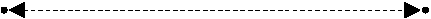
\includegraphics[scale=.7]{%
src/images/lbk-graphics/3rd-law.pdf}}; \node at (-2.75,0) {\small 
 $P$} ;
\node at (2.75,0) {\small  $Q$} ;
\end{tikzpicture}
\end{center}
\caption{}\label{fig6.11}
\end{figure}

According to the third law of Newton, the force exerted 
by $Q$ on $P$  is given by $\veca{f}_\sfx{\nnt QP} = 
-\gkk d =-\veca{f}_\sfx{\nnt PQ}$.  But the separation  
$d$ is the spatial distance between two 
\textsl{simultaneous events} on the world lines of $P$ 
and $Q$. Thus, we note that \textsl{the forces of 
action and reaction are equal and opposite and 
simultaneous} in the IRF $S$. Since simultaneity of 
events is not preserved when we go to a different IRF, 
say $S'$, the third law is not valid in  $S'$. Hence  
the third law of Newton cannot be a general law which 
is valid in all Lorentz frames. However, we can still 
keep the law in the special case when the action and 
reaction arise from the interaction of two particles in 
contact because, then, simultaneity at the same point 
of space ($\Delta\veca{r}_\sfx{PQ}=0$ in 
Eqn.\eqref{pm8}) is carried over to other Lorentz 
frames.

\vspace{-.2cm}

\section{Hyperbolic motion}
As an example of the application of the relativistic 
Newton 
law, we discuss the motion of a mass-point of 
rest-mass 
$m_0$ in a constant 3-force field $m_0 \gka\,\eye$ 
where 
$\gka$ is a {positive} constant. The relevant equation 
of 
motion is 
\begin{align}\label{pm29} 
m_0\,\dv{(\Gamma \veca{u})}{t}=m_0 \gka\,\eye, 
\end{align} 
which breaks up into the three equations
\begin{align}\label{pmx30}
\dv{(\Gamma u_x)}{t}& = \gka, 
\end{align}
\begin{align}
\dv{(\Gamma u_y)}{t}& =0,\quad\text{ and }\quad
\dv{(\Gamma u_z)}{t} =0.\label{pmx31}
\end{align}
For simplicity, we consider motion with the initial 
conditions
\begin{align}\label{pm30}
y =z=0,\; u_x=u_y=u_z=0  \text{ at }  t=0.
\end{align}
Then, Eqn.\eqref{pmx31} gives $y(t) =0$ and $ z(t) =0$ 
for 
all $t$ showing that the motion is along the $x$-axis 
of the 
frame $S$. The remaining equation \eqref{pmx30} gives
\begin{align}\label{pm31}
\Gamma u = \gka t,
\end{align}
where we have denoted $u_x$ by $u$ for simplicity. On
squaring,  Eqn.\eqref{pm31} becomes
\begin{align}\label{pm32}
\Gamma^2 u^2=u^2/(1-u^2/c^2)=  \gka ^2 t ^2.
\end{align}
Thus,
\begin{align}\label{pm33}
u=\dot{x}=\frac{\gka t}{\sqrt{1+\gka^2 t^2/c^2}}\;,
\end{align}
where we have taken the positive root  which 
corresponds to 
motion along the positive $x$-axis. Observe that 
$u\rightarrow c \text{ as } t \rightarrow \infty$. 
Thus, 
{however long we may subject a material particle to a 
constant force $m_0 \gka$, its speed $u$ remains less 
than 
$c$} (as measured in the frame $S$). Next, integrating 
Eqn.\eqref{pm33}, we get
\begin{align*}
x(t)&= \int \frac{\gka t
\,dt}{\sqrt{1+\gka^2 t^2/c^2}}+\text{const.}\notag\\&=
\frac{c^2}{2\gka}\int
 \frac{d(\gka^2
t^2/c^2)}{\sqrt{1+\gka^2t^2/c^2}}+\text{const}.
\end{align*}
We choose the initial condition $ x(0) =c^2/\gka$ to 
make 
the constant of integration zero and obtain
\begin{align}\label{pmx34}
x(t)=(c^2/\gka)\sqrt{1+\gka^2t^2/c^2}.
\end{align}
If we expand  the (relativistic) formulae 
Eqn.\eqref{pm33} 
and  Eqn.\eqref{pmx34} in a  power series of $\gka 
t/c$, 
we get
\begin{align*}
&u =\gka t -\gka^3t^3/c^2+ \dt  \\
&x(t) =x(0)+ \frac{1}{2}\gka t^2
-\frac{\gka^3t^4}{8c^2} +\dt
\end{align*}
In the limit $\gka t/c << 1 $, we may observe that 
these two
formulae reduce to their well known {Galilean 
counterparts}.

From Eqn.\eqref{pm31} and Eqn.\eqref{pm33}, we identify 
 
the factor $\Gamma$:
\begin{align}\label{pm36}
\Gamma =\gka t/u =\sqrt{1+\gka^2t^2/c^2}.
\end{align}

Next, a straight forward calculation gives $a=\dd u/ 
\dd 
t=\gka/\Gamma^3$ so that
\begin{align}\label{pm37}
\veca{a}=a\,\eye=(\gka/\Gamma^3)\,\eye,
\end{align}
is the 3-acceleration of the particle and the 
corresponding 
proper-3-acceleration of the particle (See 
Eqn.\eqref{pm17}) 
is
\begin{align}\label{pm38}
\ustar{a}=\Gamma^3 a= \gka.
\end{align}
Thus, the motion under a constant 3-force $\veca{f} 
=m_0\gka\,\eye$ may also be characterised as a motion 
with 
the constant proper 3-acceleration  $\gka =|\veca{f}| 
/m_0$. 
Also, using Eqn.\eqref{pmadd20}, we identify the 
components 
of the associated 4-acceleration:
\begin{align}\label{pm39}
A^0= \gka^2 t/c,\; \; A^1= \gka\sqrt{1+\gka^2 
t^2/c^2},\;
\; A^2=A^3=0.
\end{align}
Lastly, we rearrange Eqn.\eqref{pmx34} as
\begin{align*}
 x^2/(c^2/\gka)^2 =1+w^2/(c^2/\gka)^2,
\end{align*} 
which we recognise as the hyperbola 
\begin{align}\label{pm40}
 1&=\frac{x^2}{\gkk^2} - \frac{w^2}{\gkk^2},\quad
 \gkk^2\equiv(c^2/\gka)^2.
\end{align}
\begin{figure}[H]
\begin{center}
\begin{tikzpicture}
%   \draw[help lines,step=.25,red] (-4,-4) grid (4,4) ;
%   \foreach \y in {-4,-3.5,...,4}
%     \draw (-4.2,\y) node[left]{\tiny\y} ;
%   \foreach \x in {-4,-3.5,...,5}
%     \draw (\x,-4.2) node[below]{\tiny\x} ;
\node at (0,0) {\includegraphics[scale=1]%
{src/images/lbk-graphics/event-horizon}};
\node at (-.2,2.75) {\small  $ct$} ;
\node at (2.9,-.13) {\small  $x$} ;
\node at (2.4, -1.05){\scriptsize $\text{World-line}$} 
;
\node at (-1.4,1.1)  { \scriptsize 
$\text{Event-horizon}$} ;
\end{tikzpicture}\end{center}
\caption*{Figure 6.12:~Event horizon of the particle moving with a 
constant proper-3-acceleration}\label{fig6.12} 
\end{figure}
This is the reason why the motion under a constant  
3-force 
is also referred to as \textsl{hyperbolic motion}. In 
contrast, upon choosing $ x(0) =0$ in the Galilean 
formulae 
for simplicity, we note that the Newtonian orbit under 
a 
constant 3-force given by
\begin{align}\label{pm42}
 w^2=(2c^2/\gka)x.
\end{align}
is \textsl{parabolic}.

In passing, we may mention about another interesting 
feature 
of the hyperbolic motion. In \figref{fig6.12}, we have 
a 
parametric plot of the coordinate  pair $(ct, x(t))$ 
giving 
the world line of the particle with $y$ and $z$ 
suppressed.

It is interesting to note that the line\footnote{It is 
actually is a 3-dimensional hypersurface when $y$ and 
$z$ 
are reintroduced.} in the diagram of which $OB$ is a 
part, 
is an {event horizon} associated with the particle. 
The 
upper asymptote $OB$ is the world line of a light 
signal 
sent from $ x=0$ at $t=0$. Thus, it is impossible to 
communicate with the particle from any point on the 
$x$-axis which is behind the particle by a spatial 
distance 
$\geq c^2/\gkk$.

\section{Covariant form of Newton's law}
Observe that the relativistic Newton law 
Eqn.\eqref{pm26} 
holds in every Lorentz frame although is a 3-vector 
equation. One may wonder how a non-4-tensorial equation 
such 
as Eqn.\eqref{pm26} is actually covariant under 
Lorentz 
transformations. Now we demonstrate that there is 
nothing 
surprising about this because Eqn.\eqref{pm26} is in 
fact a 
part of a {4-vector equation}.

Multiplying both sides of Eqn.\eqref{pm26} by $\Gamma$ 
and 
using the relation $\Gamma d\tau =dt$ which is true 
along 
the world line of the particle, we write it as
\begin{align}\label{pm43}
\Gamma (\dd \veca{p}/\dd t)=(\dd \veca{p}/\dd 
\tau)=\Gamma\veca{f}.
\end{align}
The term $ (\dd \veca{p}/\dd \tau) $ in the equation 
above is 
the space part  ($ i=1,2,3 $) of the 4-vector $(\dd 
P^\gka/\dd \tau)$. Therefore, we consider the equation
\begin{align}\label{pm44}
(\dd P^\gka/\dd \tau)=F^\gka,
\end{align}
where
\begin{align}\label{pm45}
F^\gka \equiv (F^0, \Gamma \veca{f}),
\end{align}
with an {undetermined term}$ F^0 $. Clearly, if an 
$F^0$ 
could be determined such that  the $F^\gka$ in 
Eqn.\eqref{pm45} is a 4-vector, then Eqn.\eqref{pm44} 
would 
be a 4-vector equation as desired. To determine $ F^0 
$, we 
contract Eqn.\eqref{pm44} with $U_ \gka$, use the 
results 
$U^\gka U_ \gka =c^2$ and $U_ \gka A^\gka =0$ and 
obtain
\begin{align}\label{pm46}
U_ \gka F^\gka&=U_ \gka \dv{P^\gka}{\tau}
=U_ \gka \dv{(m_0U^\gka)}{\tau}\notag \\\notag 
&=U_ \gka U^\gka\,\dv{m_0}{\tau} +m_0
U_ \gka \dv{U^\gka}{\tau} \notag\\ 
&=c^2\dv{m_0}{\tau}+m_0 U_ \gka A^\gka
=c^2\dv{m_0}{\tau}.
\end{align}
Now, with \textsl{one reasonable assumption} thrown 
in, 
namely
\begin{align}\label{pm47}
\dv{m_0}{\tau}=0,\; \textsl{along the world line of the
particle},
\end{align}
we arrive at the relation
\begin{align}\label{pm48}
U_ \gka F^\gka=0.
\end{align}
Note that the assumption Eqn.\eqref{pm47} simply means 
that 
the particle has the same rest-mass $m_0$ all along 
its 
world line. Equivalently, since  $dm_0/d\tau = (\dd 
t/\dd 
\tau)(\dd m_0/\dd t)=\Gamma(\dd m_0/\dd t)$, the 
assumption 
Eqn.\eqref{pm47} also implies that {the particle has 
the 
same {identity}}, namely, its {rest-mass} $m_0$, at 
all 
times $t$. Now, we solve the equation  $U_ \gka 
F^\gka=0$ 
and obtain
\begin{align}\label{pm49}
F^0 =-\frac{U_1 F^1 +U_2 F^2 +U_3 F^3}{U_0 }
=\frac{\Gamma \veca{u}\dotp\veca{f}}{c}\,.
\end{align}
Thus,
\begin{align}\label{pm50}
F^\gka= \Gamma\left(\veca{u}\dotp\veca{f}/c, \veca{f} 
\right),
\end{align}
and with this 4-vector called the \textsl{Minkowski 
force}, 
the equation \eqref{pm44} would be 4-vector equation 
provided the Minkowski force $F^\gka$ satisfies the 
condition in Eqn.\eqref{pm48} which requires that 
\textsl{the 4-force is (Minkowski) orthogonal to 
4-velocity}. It is gratifying to note that the only 
classical 4-force known, namely the Lorentz 4-force in 
vacuum electrodynamics, satisfies this condition.

Lastly, we display the 4-vector equation 
Eqn.\eqref{pm44} in
another  equivalent form:
\begin{align}\label{pmadd53}
m_0(\dd A^\gka/\dd \tau)=F^\gka,
\end{align}
which follows because of the assumption 
Eqn.\eqref{pm47}.
Verbally  stated, this equation says:

\textsl{The product of the rest-mass and the 
4-acceleration 
of a  material particle is equal to the 4-force acting 
on 
it}.

We  may observe that we constructed the 
Eqn.\eqref{pm44} 
such that it yields the relativistic 3-vector Newton 
law in 
Eqn.\eqref{pm26} for $ i =1,2,3 $. But there is an 
extra 
equation in Eqn.\eqref{pm44}, namely its zeroth 
component:
\begin{align*}
(\dd P^0/\dd \tau) &=\Gamma (\dd P^0/\dd t)=\Gamma
[\dd (mc)/\dd t] =
\Gamma\veca{u}\dotp\veca{f}/c.
\end{align*}
What does this equation mean? To find the answer,  we 
rearrange the above equation as
\begin{align}\label{pm52}
 \dd (mc^2)=
(\veca{f}\dotp\veca{u})\,\dd t=\veca{f}\dotp 
\dd{\veca{r}},
\end{align}
where we recall that $\dd{\veca{r}}$ is the 
infinitesimal 
3-vector displacement of the particle which occurs in 
the 
infinitesimal time $ \dd t $. Thus, {the work done by 
the 
force $\veca{f}$ on the particle in moving it from 
$\veca{r}$ 
to $\veca{r} +\dd \veca{r}$ increases  the quantity $ 
mc^2$ 
associated with the particle by the differential amount 
$ 
\dd (mc^2)$}. Integrating Eqn.\eqref{pm52} from 
$\veca{r_0}$ 
to $\veca{r}$ along the space-orbit $\gkk: 
\veca{r}=\veca{r}(t)$ of the particle, we get
\begin{align}
m(\veca{r})=m(\veca{r_0})+\frac{1}{c^2}\,{}_{\gkk}
\hsn\int_{\veca{r_\sfx{0}}}^{\veca{r}}\nt \veca{f}\dotp
\dd{\veca{r}},
\end{align}
which defines the momental (or relative) mass of the 
particle as a function $  m(\veca{r})$ on its space 
trajectory $\gkk$. This relation also implies that the 
work 
done by the force in moving the particle from  
$\veca{r_0}$  
to $\veca{r}$ 
 
along the path  $\gkk$ appears as the change  $\Delta 
m\equiv m(\veca{r})-m(\veca{r_0})$ in the momental  
mass of 
the particle. This connection between the change in 
the 
momental mass $ m(\veca{r})$ of the particle and the 
work 
done by the 3-force field $\veca{f}$ on it, both 
defined only 
on  $\gkk$, is the extra information on the particle's 
motion that is contained in the zeroth-component of 
the 
4-vector equation of motion Eqn.\eqref{pm44}.

When the 3-force field \ $\veca{f}$ is 
\textsl{conservative}, 
i.e., if $\veca{f}= - \veca{\nabla} \varphi$, then 
Eqn.\eqref{pm52}
becomes
\begin{align*}
 \dd (mc^2)=\veca{f}\dotp\dd{\veca{r}}=-\veca{\nabla}
\varphi\dotp\dd{\veca{r}}=-\dd\varphi,
\end{align*}
so that
\begin{align}
 mc^2+\varphi=\text{constant } \equiv E,
\end{align}
which gives an integral of motion. The quantity 
$E=mc^2+\varphi$, called \textsl{the total 
relativistic 
energy of the particle} has the same value at all 
points of 
the space orbit of $\gkk$ of the particle.

\subsection{Lorentz transformation of 3-force}
The 3-force $\veca{f}$ which occurs in the 
relativistic 
Newton law \eqref{pm26} has no simple transformation 
property under a  Lorentz transformation. 
\textsl{Unlike its 
Newtonian counterpart, it is not unchanged under a 
transformation form one inertial (i.e. Lorentz) frame 
to 
another.} To see this, we obtain its transformation 
rule by 
appealing to the fact that the 3-force vector 
$\veca{f}$ is 
part of the 4-force, or Minkowski force, $F^\gka$ given 
in 
Eqn.\eqref{pm50}. Observe that the equation (6.1) gives 
the 
transformation rule of a general contravariant 4-vector 
 
$A^\gka\equiv (A^0,\veca{A})$ under a general boost 
\eqref{pmadd3}and \eqref{pmadd4}. If we replace $A^0$ 
and 
$\veca{A}$ in the equation (6.1) by $\Gamma 
(\veca{u}\dotp\veca{f})/c$ and $\Gamma \veca{f}$ 
respectively, 
we get
\begin{align}
&\Gamma' \pvec{f}
% =\Gamma\veca{f}+\big[-\gkg \Gamma
% (\veca{u}\dotp\veca{f})/c
% 
+(\gkg-1)(\veca{\gkb}\dotp\Gamma\veca{f}/\gkb^2)\big]
\veca{\gkb
}
\notag\\
&=\Gamma\Big[\veca{f}-\gkg
(\veca{u}\dotp\veca{f})\veca{\gkb}/c+(\gkg-1)(\veca{
\gkb}\dotp 
\veca{f}
/\gkb^2)\veca{\gkb} \Big].
\end{align}
Now, we may substitute for $\Gamma' /\Gamma$ above from
Eqn.\eqref{6.13x} and obtain
\begin{align}
\pvec{f}=\frac{\veca{f}-\gkg
(\veca{u}\dotp\veca{f})\veca{\gkb}/c+(\gkg-1)(\veca{
\gkb}\dotp 
\veca{f} /\gkb^2)\veca{\gkb}}{\gkg\big(1-\veca{\gkb}
\dotp\veca{u}/c\big) }.
\end{align}
which is required \textsl{law of transformation of the 
relativistic 3-force} $\veca{f}$ under the general 
boost  
\eqref{pmadd3} and \eqref{pmadd4}.

\newpage

\section{Relativistic collision-kinematics}
\begin{small}
\begin{quote}
\hbf{Reference}

[1]~David J. Griffiths, {Introduction to\\ Elementary
Particles}, 1987, John Wiley \& Sons Inc.\\ New York
\end{quote}
\end{small}

\hbf{Notation}: In this section, we work in 
\textsl{Natural 
Units} in which  $ c=1$.  `Euler-Script' characters' 
such as $\EuScript{A},\EuScript{B},  \EuScript{C}..$,  
denote  4-vectors and the usual upper case  characters 
with suffixes such as $A^\gka, \,B_ \gka\dt$, denote 
their 
contra and covariant components in a Lorentz frame. 
Lower 
case characters such as $\veca{u},\, \veca{v}, \dt$, 
with an 
arrow above, denote 3-vectors, as usual. The Cartesian 
components of $\veca{u}$ are denoted by 
$u_x,\;u_y,\;u_z$ 
and 
$u$ denotes $ |\veca{u}|$. The Minkowski scalar product 
of 
the $\EuScript{A}$ and $\EuScript{B}$ is defined  by
\begin{align}\label{pm53}
&\EuScript{A}\minp\EuScript{B}\equiv
\eta_{\gka\gkb}{A}^\gka {A}^\gkb = A_ \gka B^\gka= 
\eta^{\gka\gkb}{A}_ \gka B_\gkb,\notag\\
&\eta_{\gka\gkb}=\eta^{\gka\gkb}=\diag(1,-1,-1,-1).
\end{align}

Recall that the (timelike) 4-momentum vector of a 
particle 
of rest-mass $ m_\sfx{A}$ moving with the 3-velocity $ 
\veca{u}_\sfx{A}$ is
\begin{align}\label{pm54}
&P_\sfx{A}^\gka =(E_\sfx{A},\veca{p}_\sfx{A})=
\Gamma_\sfx{A} m_\sfx{A}(1, \veca{u}_\sfx{A}),\;
E_\sfx{A}^2> p_\sfx{A}^2, \notag\\&\text{where 
}\Gamma_\sfx{A} \equiv  (1-u_\sfx{A}^2)^{-1/2},
\end{align}
\subsection{The law of conservation of  4-momentum}
In  collision problems, a {photon} is pictured as a 
\textsl{localised particle} with  a \textsl{null} 
4-momentum 
$\hslash \EuScript{K}$ given by
\begin{align}\label{pm55}
\hslash{K}^\gka=\hslash\omega\,(1,\hat{\gkk}),
\;\;\omega^2=\gkk^2,
\end{align}
where $\omega$ is the {(angular) frequency} of the 
photon 
and  $\hat{\gkk}$ is its {direction of propagation} in 
space.

The law of conservation of 4-momentum is the basic law 
of
collision theory and states that in every inertial 
(Lorentz)
frame,
\begin{align}\label{pm56}
\sum_{A=1}^n {P'}^\gka_\sfx{A}=\sum_{A=1}^n
P_\sfx{A}^\gka,
\end{align}
where  ${P}'^\gka_\sfx{A}$ are the 4-momenta of the 
$n$ 
colliding particles \textsl{after}  collision and 
$P_\sfx{A}^\gka$ are the corresponding 4-momenta 
\textsl{before} collision.

\exm  Two objects, each of rest mass $ m $, stick 
together 
to form a single object of rest mass $M$ after a 
head-on 
collision. Assuming that both the objects of rest mass 
$m$ 
were travelling with the speed $3/5$, find $M$.
\soln
{Before collision }:
\begin{align}\label{pm66}
& \Gamma_1=\Gamma_2=5/4, \notag \\
&\EuScript{P}_{tot}=\EuScript{P}_1+\EuScript{P}_1
=(5m/4) (1, \veca{p})+
(5m/4) (1, -\veca{p})\notag \\&=(5m/2, \veca{0}).
\end{align}
{After collision }:
\begin{align}\label{pm67}
{\EuScript{P}'}_{tot}=(M,\veca{0}).
\end{align}
Equating $\EuScript{P}_{tot}$ and $ 
{\EuScript{P}'}_{tot}$, 
we get $ M=5m/2 $.  \ebx

\subsection{The centre of momentum frame}
Collision problems are often studied in a convenient 
Lorentz frame called the \textsl{Centre of Momentum 
Frame} (CMF) or the \textsl{Centre of Inertia Frame}, 
in which the total  3-momentum of the system is zero.

\begin{figure}[H]
\begin{center}
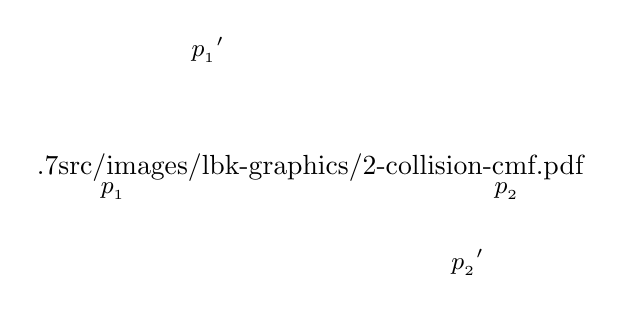
\begin{tikzpicture}
% \node at (0,0){\includegraphics[scale=.7]{%
% lbk-graphics/2-collision-cmf.pdf}};
\node at (0,0) %
{\ingra{.7}{src/images/lbk-graphics/2-collision-cmf.pdf}};
\node at (-2.5,-.3) {\small  $\veca{p_{_1}}$} ;
\node at (2.5,-.3) {\small  $\veca{p_{_2}}$} ;
\node at (-1.3,1.5) {\small  $\veca{p_{_1}}'$} ;
\node at (2, -1.2) {\small  $\veca{p_{_2}}'$} ;
\end{tikzpicture}
\caption*{Figure 6.13:~Two particle collision in the 
centre of momentum frame} \label{fig6.13}
\end{center} 
\end{figure}
Then, obviously,  the time-axis of the centre of 
momentum 
frame would be along the (time-like) total 4-momentum 
of the 
system. We denote all variables in the centre of 
momentum 
frame by the suffix ``$c$''. Then, we have,  in a 
two-particle collision  in the centre of momentum 
frame,
\begin{align*}
&P^\gka_{1c}=(E_{1c}, \veca{p}_{1c}),\quad 
P^\gka_{2c}=(E_{2c},
-\veca{p}_{1c}),
\end{align*}
\begin{align*}
 &{P}\,'^\gka_{1c}=({E}\,'_{1c},
{\veca{p}\,'}_{1c}),\quad 
{P}\,'^\gka_{2c}=({E}\,'_{2c},
-{\veca{p}\,'}_{1c}),\\
&P^\gka_{1c}+P^\gka_{2c}
=(E_c, \veca{0})={P}\,'^\gka_{1c}+{P}\,'^\gka_{2c},  
\text{ where } \\
& E_c \equiv E_{1c}+E_{2c}={E}\,'_{1c}+{E}\,'_{2c}.
\end{align*}

\subsection{Kinematics of disintegration}
In the Lorentz frame $S$, a particle of (rest) mass 
$M$ 
decays (i.e., disintegrates) {at rest} into two 
particles 
of 
(rest) masses $m_1$ and $m_2$. Clearly, the Lorentz 
frame 
$S$ is the centre of momentum frame of the system. In 
this 
centre of momentum frame $S$, the conservation law 
\begin{align}\label{pm57}
 P^\gka_M = P^\gka_1 + P^\gka_2,
\end{align}
i.e., $ (M,\veca{0})=(E_{1c},\veca{p}_{1c}) 
+(E_{2c},\veca{p}_{2c}) $, yields the following two 
equations:
\begin{align}\label{pm58}
M=E_{1c}+E_{2c},
\end{align}
\begin{align}\label{pm59}
\veca{p}_{1c}=-\veca{p}_{2c}.
\end{align}

From \eqref{pm58}, we infer that
\begin{align}\label{pm60}
M=m_1\Gamma_1+m_2\Gamma_2>m_1+m_2,
\end{align}
which is a \textsl{necessary condition} for the 
spontaneous 
decay of $M$ from rest. The particle $M$ is 
\textsl{stable} 
against {spontaneous decay} if $ M<m_1+m_2$. To induce 
 
decay of $M$ at rest into $m_1$ and $m_2$, one must 
supply 
the energy $ m_1+m_2-M $ called the \textsl{binding 
energy} 
of $M$. The quantity $\Delta M \equiv M - m_1-m_2$ is 
called the \textsl{mass-excess}.

\subsection{Individual energies in a two-body collision}
Rewriting  Eqn.\eqref{pm57} as $P^\gka_1 = P^\gka_M 
-P^\gka_2$ and forming the squared norm of $P^\gka_1$, 
we get $  P^\gka_1 P_{1i} = P^\gka_M P_{Mi} + P^\gka_2 
P_{2i} - 2 P^\gka_M P_{2i}$ which simplifies to
\begin{align}\label{pm61}
m_1^2=M^2 + m_2^2 -2ME_{2c}.
\end{align}
Thus,
\begin{align}\label{pm62}
E_{2c}=\frac{M^2 + m_2^2 -m_1^2}{2M}.
\end{align}
Similarly, solving Eqn.\eqref{pm57} for $P^\gka_2$ and 
taking the Min  -kowski  products, we obtain
\begin{align}\label{pm63}
E_{1c}=\frac{M^2 + m_1^2 -m_2^2}{2M}.
\end{align}

Sometimes it is more useful to have expressions for the
(relativistic) kinetic energies $T_{1c}$ and $T_{2c}$ 
of the
decay products:  We have
\begin{align}\label{pm64}
T_{1c}&=E_{1c}-m_1 \notag \\&=[M^2 + m_1^2 -m_2^2
-2Mm_1]/2M \notag \\&=\left[(M-m_1)^2  
-m_2^2\right]/2M\notag
\\&=(M-m_1-m_2) (M-m_1+m_2)/2M\notag \\
&=\Delta M \left\{2M-(M-m_1-m_2) 
-2m_1\right\}/2M\notag\\
&=(1-m_1/M- \Delta M/2M))\Delta M.
\end{align}
Similarly, we  obtain the kinetic energy of the second 
 
particle:
\begin{align}\label{pm65}
T_{2c}=\left( 1-m_2/M - \Delta M/2M\right)\Delta M.
\end{align}

\subsection{The Compton effect}
It is convenient to revert back from natural units 
($c=1$) 
to standard SI units ($c\neq1$) in this discussion. 
Consider 
the collision of a photon with a free electron (of 
rest-mass 
$m_0$) at rest in the Lorentz frame $S$. Let $K^\gka= 
(h\nu/c)(1,\hat{\gkk})$ and $P^\gka=(m_0 c,\veca{0})$ 
be the 
4-momenta of the photon and the electron {before} and 
$K'^\gka=(h\nu\,'/c)(1,\hat{\gkk}\,') $ and 
$P^\gka=m_0\Gamma (c,\veca{u})$ be the corresponding 
\break 4-momenta 
{after} the collision. Then, we have, by the law of 
conservation of 4-momentum,
\begin{align}\label{pm68}
& m_0 c +h\nu/c=m_0\Gamma c +h\nu'/c\\
& (h\nu/c)\hat{\gkk}=(h\nu\,'/c) \hat{\gkk}\,'
+m_0\Gamma\veca{u}. \label{pm69}
\end{align}

Following Synge, [{J. L Synge, Relativity: The Special 
Theory, North Holland, Amsterdam, 1972, p.194.}], we 
introduce the notation \begin{align}\label{pm70} 
\xi=\nu\,'/\nu,\quad \gka=h\nu/m_0c^2. \end{align} 
Using 
this notation, the equations Eqn.\eqref{pm69} and  
Eqn.\eqref{pm68}  take the form
\begin{align}\label{pm71}
\Gamma \veca{u}/c & =\gka\hat{\gkk}-\gka \xi
\hat{\gkk}\,', \\ \Gamma-1&=\gka(1-\xi).\label{pm72}
\end{align}
\begin{figure}[H]
\begin{center}
\begin{tikzpicture}[>=stealth',scale=1.2]
\coordinate (O) at (2.5,2.5);
\coordinate (A) at (4.5,2.5) ;
\coordinate (B) at (6,3.5);
\coordinate (C) at (6,.8) ;
\coordinate (X) at ($(O)!.5!(A)$) ;
\coordinate (Y) at ($(A)!.7!(B)$) ;
\coordinate (Z) at ($(A)!.6!(C)$) ;
\draw[very thick ] (A) -- (O) ;
\draw[very thick ,->]  (1,2.5)-- (O);
\draw[dashed,->] (A) --(6.5,2.5) ;
\draw[dashed,->] (A) --(4.5,4) ;
\draw[above] (4.5,3.95)node{\small $\hat{n}$} ;
\draw[right] (6.5,2.5)node{\small $\hat{\gkk}$} ;
\draw[very thick] (A) -- (B) ;
\draw[very thick,->] (A) -- (Y) ;
\draw[very thick] (A) -- (C) ;
\draw[very thick,->] (A) -- (Z) ;
\draw[above](2.5,2.5) node
{\small $\hbar \veca{\gkk}{\;}$};
\draw[left](Y) node {\small $\hbar \veca{k'}{\;\;}$};
\draw[left](Z) node {\small $\veca{p}\;\;$};
\draw[right] (4.75,2.63) node {\small $\theta$} ;
\draw[right] (4.73,2.27) node {\small $\varphi$};
% \shadedraw[ball colour=black] (A) circle (1.5mm);
% \shadedraw[ball colour=black] (C) circle (1.5mm);
% \shadedraw[ball colour=yellow] (B) circle (1mm);
% \shadedraw[ball colour=yellow] (2.25,2.5) circle 
(1mm);
\end{tikzpicture}
\caption*{Figure 6.14:}\label{fig6.14}
\end{center}
\end{figure}
Squaring Eqn.\eqref{pm71} we get
\begin{align}\label{pm73}
& \Gamma^2 \veca{u}\dotp \veca{u} /c^2  
=\Gamma^2-1=\gka^2(1-2\xi\cos\theta+\xi^2),\notag\\
& \pvec{\gkk}\dotp \veca{\gkk} =\cos\theta,
\end{align}
where we have used the relation $u^2/c^2 
=1-1/\Gamma^2$. 
Then, using  Eqn.\eqref{pm72}, we get
\begin{align}\label{pm74}
\Gamma+1 =\frac{\Gamma^2-1}{\Gamma-1} 
=\frac{\gka(1-2\xi\cos\theta+\xi^2)}{1-\xi}
\end{align}
Now subtracting Eqn.\eqref{pm72} from Eqn.\eqref{pm74}, 
we 
get\\
\vspace*{-1\bsk}\begin{align*}
 2&=\frac{\gka(1-2\xi\cos\theta+\xi^2)
-\gka(1-2\xi+\xi^2)}{1-\xi}\\ &=
2\xi\gka(1-\cos\theta)/(1-\xi).
\end{align*}
Thus,
\begin{align}\label{pm75}
(1/\xi)=\nu/\nu\,'=\gkl\,'/\gkl=1+\gka(1-\cos\theta).
\end{align}
This gives the \textsl{wavelength of the photon after 
the 
collision}:
\begin{align}\label{pm76}
 \gkl\,'&=\gkl+\gkl\gka(1-\cos\theta)
\equiv \gkl+\gkl_e (1-\cos\theta),
\end{align}
where
\begin{align}\label{pm77}
\gkl_e\equiv  (h/m_ 0c),
\end{align}
is called the \textsl{Compton wavelength of the 
electron}.

\section{Appendix 6A: The Newtonian regime in physics}
\index{Newtonian ! regime}

Before leaving this chapter, we make a few remarks on 
the
Newtonian assumptions listed in \S\,1.4. Today, we know 
that
all these postulates of Newtonian physics, namely, 
absolute
space, absolute time, absolute force, absolute 
velocity,
absolute acceleration, absolute mass, instantaneous 
forces
or actions-at-a-distance, are rejected by the special 
theory
of relativity. Furthermore, the notions of 
free-particles
and global Lorentz frames are dislodged by
\textsl{Einstein's equivalence principle} which shows 
that
the special theory of relativity is valid only in a 
locally
Lorentz frame in spacetime. So, quite naturally, the 
beginner student is left wondering why should one 
study 
Newtonian mechanics  founded on such (ultimately) 
unacceptable concepts. To reassure the student of the 
need 
for studying Newtonian mechanics, we note that the 
special 
relativistic laws reduce to the corresponding 
Newtonian 
physical laws in the \textsl{Newtonian limit of 
$c\rightarrow \infty$ } where $c$ is the speed of light 
in 
vacuum. The passage to the the limit $c\rightarrow 
\infty$ 
\textsl{effectively}\footnote{Note the word 
\textsl{effectively} that is used here. A word of 
caution to
the student: The assumption that the speeds involved 
are
\textbf{sufficiently small} compared to the finite 
speed
$c$ does not \textbf{does not} bring back the absolute 
nature of time or the instantaneous nature of the 
forces. 
To get these, one must let $c\rightarrow \infty$ which 
is 
the \textbf{true Newtonian limit}.} means that all the 
speeds involved under a given physical context are 
very 
small compared to $c \sim \SI{3e8}{m/s}$. This, in 
turn 
requires that forces involved under the same physical 
context, if any, are sufficiently weak, or, act for 
such 
short intervals of time so that they do not accelerate 
particles to speeds comparable to $c$. Therefore, 
\textsl{the laws of Newtonian mechanics hold (to a 
very 
good approximation) in the limit of low speeds and 
weak force fields}. The regime of low speeds and weak 
force 
fields is called the \textsl{Newtonian regime in 
physics}.

Because our day-to-day experience in this physical 
world 
(normally) corresponds to those involving low speeds 
and 
weak force fields, we may ``\textsl{safely}'' use the 
Newton 
laws in physics. Of course, there are many important 
physical situations, which may be called 
\textsl{non-Newtonian} or \textsl{relativistic} 
situations, 
in which \textsl{we should not rely upon the Newton 
laws}. A 
discussion of a few of such non-Newtonian, or, 
relativistic, 
situations is precisely the matter of discussion in 
this 
book.

\section{Appendix 6B: Inertial frame in the\\ special 
theory 
of relativity}
\index{inertial frame ! definition of} In 
pre-relativity 
physics, or, to be precise, in the  Newtonian regime 
in 
physics, a frame in which the three laws of motion hold 
is 
defined as an inertial frame. Then (Cf. \S~1.6)),  
according 
to the principle of Galilei relativity, \textsl{every 
Galilei frame would be an inertial frame}. Later, in 
the 
special theory of relativity, we postulate the 
existence of 
a  class of frames of reference called \textsl{Lorentz 
frames}, in each one of which all the  
non-gravitational 
laws of physics, including the first and second laws 
of 
Newton (albeit in a certain modified  \ie, 
relativistic, 
form), hold. In other words, in the special theory of 
relativity,  we  identify a Lorentz frame as an 
inertial 
frame. It may appear inconsistent that we define an 
inertial 
frame as a Galilean frame in the  Newtonian regime and 
as a 
Lorentz frame in special relativity physics. However, 
this 
apparent inconsistency disappears once we note that a 
Lorentz transformation reduces to a Galilei 
transformation 
in the Newtonian limit of $c\rightarrow \infty$.

As already observed, a Galilei frame is an inertial 
frame 
{to a sufficient degree of accuracy}. So, in the 
Newtonian 
regime, we use a Galilei transformation to transform 
from 
one inertial frame to another  However, in the  
relativistic 
regime, ``Lorentz replaces  Galilei'':  Then, a 
Lorentz 
frame is (correctly) identified as an inertial frame. 
Now, we may borrow the Einsteinian definition of a 
Lorentz 
frame from \S~4.1.1 and use it to define an inertial 
frame as follows:

\dfnarg{Inertial frame} A global Cartesian coordinate 
system 
in the Minkowski spacetime relative to which the speed 
of 
light in vacuum is isotropic and has the universal 
value $c$ 
is an inertial frame. 

Consequently one has to use a Lorentz transformation 
(and 
not a Galilei transformation !) to transit from one 
inertial frame to another. The definition~6.7 makes
the phrases 'inertial  frame' and 'Lorentz frame' 
synonymous. Also, the definition~6.7 of an inertial 
frame, 
unlike its Newtonian counterpart (cf. \S~1.6), is not 
tied 
up with the notion of \textsl{force}, or, more 
precisely the 
postulate of a  \textsl{free particle}.  However, even 
this 
definition~6.7 also runs into trouble when we take 
into 
account the Einstein equivalence principle according 
to 
which, the notion of a global inertial frame (\ie, an 
inertial frame covering the whole of spacetime) is  
untenable. Without entering into a further discussion 
of the 
equivalence principle here, we simply mention that the 
equivalence principle permits identifying a local (\ie, 
not 
global) coordinate system (i.e., a coordinate system 
which 
covers a small region of spacetime around a spacetime 
event 
of interest) which is {inertial} to a desired degree 
of 
(experimental, or measuremental) accuracy. 

\section{Appendix 6C:  Time-interval\\ transformations}

Here, in this appendix, we revisit the problem of the 
Lorentz transformation of time-intervals in special 
relativity and show that there exist a whole class of 
formulae, which we may call as \textsl{time-stretching 
formulae}, each one of which  \textbf{\textsl{looks}} 
exactly like the well known time-dilation formula in 
special 
relativity. Therefore, \textsl{it is  important for a 
student to recognise the difference  between the 
Einstein 
time-dilation formula and a general time-stret-\break ching 
formula}. Moreover, occasionally [see, for example, 
Griffiths, Ref. 1, pp. 483-491], a time-stretching 
formula 
has been mistaken for the time-dilation formula in the 
literature and we also wish to draw the attention of 
the 
student such  instances.

The following discussion is based on the general 
\textsl{time-interval transformation formula} (See 
\eqref{pmadd4a})
\begin{align*}
c\Delta t' = \gkg (c\Delta t
- \veca{\gkb} \dotp \Delta \veca{r}),
\end{align*}
in which $\Delta t'$ and $\Delta t$ are the 
time-intervals 
between a  given pair of events, in two inertial frames 
$S$ 
and $S'$ connected by the  general boost in 
Eqn.\eqref{pmadd3}. 
\textsl{We observe that the Einstein 
time-dilation-formula, 
the Doppler formula and the relativity of simultaneity, 
all 
follow from the time-interval formula when one the two 
frames in it is \textsl{adapted} to the underlying 
event-pair}. We also discuss the interesting special 
case 
$\Delta t' = \gkg \Delta t$ of the time-interval 
transformation formula obtained by setting 
$\veca{\gkb} 
\dotp 
\Delta \veca{r}=0$ in it and argue why it is really 
\textsl{not} the Einstein time-dilation formula. 
Finally, 
we 
present some examples which involve material particles 
instead of light rays, and highlight the utility of 
time-interval transformation formula as a 
calculational 
tool 
in the class room.

It is satisfying that this discussion brings out the 
utility 
of the general boost \eqref{pmadd3} (and the 
time-interval 
formula) in clarifying certain misunderstandings 
concerning 
the derivation of the Einstein time-dilation formula 
for 
the 
beginner student.

\hbf{Notation and convention}
As in the rest of the book, $\mathbb{M}$ denotes the 
Minkowski  spacetime. We work in signature $ +--- $. 
Events 
in $ \mathbb{M}$ are denoted by Euler-Script 
characters 
such 
as $ \EuScript{P}_1$ and $\EuScript{P}_2$. Latin 
suffixes 
are used for the space-range 1,2,3 and Greek suffixes 
for 
the spacetime range 0,1,2,3. $ S : \{ct, x, y, z\}$ and 
 
$S' 
: \{ct', x', y', z' \}$ are two inertial coordinate 
systems 
in $\mathbb{M}$. An event, say $\EuScript{P}_1$, has 
the 
coordinates $(ct_1,x_1,y_1,z_1)  \equiv 
(ct_1,\veca{r_1})$ 
in 
the inertial frame $S$ and the coordinates  
$(ct'_1,x'_1,y'_1,z'_1)\equiv (ct'_1,\pvec{r_1}),$ in 
the 
inertial frame $S'$. The standard symbols $\gkb$ and 
$\gkg$ 
denote $v / c$ and  $1/ \sqrt{1 -v^2 / c^2}$.

\subsection{Lorentz transformation of  time-intervals}
Recall that an inertial frame is essentially a set of 
devices which enable setting up a pseudo-Cartesian 
coordinate system covering the whole of the Minkowski 
spacetime $\mathbb{M}$. In a given inertial frame, say 
$S$, 
every event  $\EuScript{P}$ is associated with a 
unique 
quadruplet $(ct,x,y,z)$ of pseudo-Cartesian 
coordinates. 
Let $\{\EuScript{P}_1, \EuScript{P}_2\}$ be a given 
pair of 
events with $S$-frame spacetime coordinates 
$(ct_1,\veca{r_1})$ and $(ct_2,\veca{r_2})$. Further, 
let 
$\EuScript{P}_2$ occur later than $\EuScript{P}_1$ in 
$S$. 
Then, the displacement 4-vector between them is given 
by  
\begin{align*}
 (ct_2-ct_1, x_2-x_1,y_2-y_1,z_2-z_1) \equiv 
(c\Delta 
t_\sfx{12},\Delta x_\sfx{12}, \Delta y_\sfx{12}, 
\Delta 
z_\sfx{12}),
\end{align*}
where we may remember that we have 
conveniently  chosen $\Delta t_\sfx{12} > 0$ in the 
$S$-frame.

Events $\EuScript{P}_1$ and $\EuScript{P}_2$ are said 
to be 
\textsl{timelike-separated}, \textsl{null-separa\break ted}, 
or 
\textsl{spacelike-separated}, according as
\begin{align*}
c^2\,\Delta t_\sfx{12}^2-\Delta
x_\sfx{12}^2-\Delta y_\sfx{12}^2-\Delta
z_\sfx{12}^2 \gtreqqless 0.
\end{align*}

Further, we need the following lemmas\footnote{These 
are 
essentially the lemmas 7.9, 7.10 and 7.10 which are 
proved 
in the following chapter~7. Combined with the evident 
observation that a pair of events, timelike-separated, 
null-separated or, spacelike-separated, define a 
corresponding timelike/null/spacelike 4-vector, the 
lemmas 
7.9, 7.10 and 7.10 become, respectively, the lemmas 
6.1, 
6.2 
and 6.3.} concerning pairs of events in $\mathbb{M}$:

\lem  A pair of  timelike-separated events is 
\textsl{contiguous} (i.e., they occur at the same 
spatial 
point) in an appropriate inertial frame called the 
canonical 
inertial frame (or, the proper-frame) of  the  
timelike-separated event-pair.

\lem  A pair of spacelike-separated events is 
\textsl{simultaneous} (i.e., they occur at the same 
instant) 
in an appropriate canonical inertial frame of the 
spacelike-separated event-pair.

\lem A pair of null-separated events has space and 
time 
separations which are related by $ c\,\Delta t_\sfx{12} 
= | 
\Delta \veca{r}_\sfx{\nnt 12} |$ in \textsl{every} 
inertial 
frame.

\begin{figure}[H]
\begin{center}
\begin{tikzpicture}
%   \draw[help lines,step=.25,red] (-4,-4) grid (4,4) ;
%   \foreach \y in {-4,-3.5,...,4}
%     \draw (-4.2,\y) node[left]{\tiny\y} ;
%   \foreach \x in {-4,-3.5,...,5}
%     \draw (\x,-4.2) node[below]{\tiny\x} ;
\node at (0,0)
{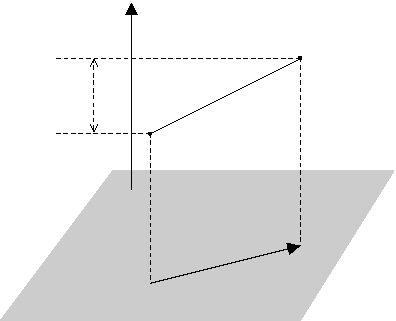
\includegraphics[scale=1]{%
src/images/lbk-graphics/st-splitting-bw.pdf}};
\node at (-1.5,1.15) {\small  $\Delta t$} ;
\node at (-1.2,2.7) [above]{\scriptsize  
\text{Time-axis}} ;
\node at (-.8,.5) [above]{\small $P$} ;
\node at (1.7,1.7) [above]{\small $Q$} ;
\node at (-1.4,-.8) [above]{\small $O$} ;
\node at (.5,-1.7) [above]{\small $\Delta\veca{r}$} ;
\node at (-1.4,-2.8) [above]{\scriptsize \text{A 
space-section}};
\end{tikzpicture}
\end{center}
\caption*{Figure 6.15:~ Time-space splitting of a spacetime 
interval}\label{fig6.15}
\end{figure}
In what follows, we use the rule for transforming the 
time-interval between an (arbitrary) event-pair in one 
inertial frame $S:\{x^\mu\}$ to that in another 
inertial 
frame  say, $ S':\{x'^\mu\}$. Since we do not want to 
restrict to any particular direction for the relative 
motion 
between the frames $S$ and $S'$, we consider $S$ and 
$S'$ 
to 
be connected by a \textsl{general Lorentz boost} (see 
Eqn.\eqref{pmadd3})
\begin{align}\label{1}
x'^\mu = \mtud{L} {\mu} {\nu}x^\nu,
\end{align}
where the Lorentz-matrix $(\mtud{L}{\mu}{\nu})$ has the
elements
\begin{align} \label{2}
\mtud{L}{0}{0} &  = \gkg, \; \;
\mtud{L}{0}{i}  = \mtud{L}{i} {0}= - \gkg \gkb_{i}, 
\noindent\\
\mtud{L}{i} {j}&= \delta_{ij} + (\gkg - 1) \gkb_{i}
\gkb_{j} /\gkb^2,
\end{align}
in which $c \veca{\gkb} = c (\gkb_1\eye  + \gkb_2 \jay 
+ 
\gkb_3\kay )$ is the constant 3-velocity of $S'$ 
relative 
to $S$, $\veca{\gkb} =  \gkb\, \hat{\gkb}$ and $\gkg = 
(1 - \gkb^2)^{- 1 / 2}$.

Using Eqn.\eqref{2}, we are again led to 
\eqref{pmadd4a} 
which connects the differences $\Delta 
t'_\sfx{12}=t'_2-t'_1$  and $\Delta 
t_\sfx{12}=t_2-t_1$ for two arbitrary events 
$\EuScript{P}_1$ and $\EuScript{P}_1$ with coordinates 
$(ct_1,\veca{r_1})$ and $(ct_2,\veca{r_2})$ in $S$: We 
note 
here this important relation \eqref{pmadd4a} for 
future 
reference:
\begin{align} \label{6.129}
\Delta t'_\sfx{12}  =\gkg \left[\Delta
t_\sfx{12}-(\veca{\gkb}/c)\, \dotp\Delta
\veca{r}_\sfx{\nnt 12}\right].
\end{align}
This equation which may be called \textsl{the general  
time-interval transformation law}, is our \textsl{key 
equation}. In the following paragraphs, taking one of 
the 
two inertial frames in Eqn.\eqref{6.129}, say $S$, to 
be 
the 
canonical frame in the cases of timelike- and 
spacelike-separated event-pairs, we determine the 
resulting 
``canonical\break forms'' of  Eqn.\eqref{6.129}. 

In the remaining case of the null-separated 
event-pair, 
because the speed of light is isotropic and has the 
same 
value in all inertial frames, it may appear that  
Eqn.\eqref{6.129} has no special canonical form. But 
we 
shall 
see that the Doppler-frequency formula is indeed a  
canonical form associated with Eqn.\eqref{6.129}. 
These 
observations show how the intrinsic nature of  
Eqn.\eqref{6.129} 
depends on the invariant-type of the event-pair 
considered.

\subsection{Timelike-separation: Time-dilation}
Let the frame $S$ be a canonical frame of the 
timelike-separated event-pair $\{\EuScript{P}_1, 
\EuScript{P}_2 \}$. Then, in $S$, $\Delta 
\veca{r}_\sfx{\nnt 
12} = \veca{r_2}-\veca{r_1}=0$ and the two events 
$\EuScript{P}_1$  and $\EuScript{P}_2$ have a 
\textsl{proper 
time-interval}$ \Delta t_\sfx{12} \equiv \Delta 
\tau_\sfx{12} >0 $ separating them. Thus,  
Eqn.~\eqref{6.129} 
takes the canonical form \begin{align}\label{4} \Delta 
t'_\sfx{12} =\gkg \Delta \tau_\sfx{12}, \end{align} 
which 
we 
recognise as the familiar \textsl{Larmor-Einstein  
time-dilation formula} \eqref{pm9} discussed earlier 
in 
\S6.9.

\subsection{Null-separation: Doppler formula}
Recall Lemma~6.3 for a null-separated pair of events. 
It 
says that there is no canonical Lorentz frame for a  
null-separated event-pair. (Or, we may say that every 
inertial frame is ``equally canonical'' for a 
null-separated 
event-pair.) So, let $\Delta \veca{r}_\sfx{\nnt 12} | = 
c\, 
\Delta t_\sfx{12}>0$, in $S$ for a given 
null-separated-pair 
of events $\{\EuScript{P}_1,\EuScript{P}_2\}$.  Then, 
in 
this case, the time-interval transformation  
\eqref{6.129} 
may also be written as
\begin{align}\label{5}
\Delta t'_\sfx{12} & ={\gkg}\, \Delta t_\sfx{12}
\left(1-{\gkb}\cos{\theta}\right),
\end{align}
where $\theta$ is the angle between the 3-vectors
$\Delta\veca{r}_\sfx{\nnt 12}$ and $\veca{\gkb}$ in 
$S$.

It is interesting to note the form assumed by  
Eqn.\eqref{5} when it is applied to a 
``light-particle'' 
(mono  -chromatic light wave) and its (material-point) 
source.  For the light-particle, we take 
$\{\EuScript{P}_1,\EuScript{P}_2\}$ to be a pair of  
null-separated events on its (null) world line.  
Although 
there is no canonical frame for a light-particle (in 
the  
sense of Lemma~6.3), we do have a canonical frame 
(rest 
frame) for its (material-point) source which we may 
take as 
the frame $S$ in Eqn.\eqref{5}. We take the 
time-interval  $\Delta t_\sfx{12} \equiv T>0 $ as the 
\textsl{period} of the photon (wave) (more specifically 
the 
\textsl{proper-period}) in $S$ in which its source is 
at 
rest. Then, $\nu =1/T $ is the 
\textsl{proper-frequency} 
and 
$\nu' =1/T'=1/\Delta t'_\sfx{12}$ given by 
Eqn.\eqref{5} is 
its \textsl{relative-frequency} in the frame $S'$, in 
which 
the source has a  uniform velocity $c\veca{\gkb}$. 
Now, 
Eqn.\eqref{5}, re-written in  terms of frequencies of 
the 
photon in the two frames, is
\begin{align}\label{6}
\frac{\nu'}{\nu}&
=\frac{\sqrt{1-v^2/c^2}} 
{\left(1-{\gkb}\cos{\theta}\right)},
\end{align}
which is the \textsl{relativistic Doppler formula} [see 
for 
example Landau and Lifshitz, Ref.~5, pp.116-17]. Here, 
in  Eqn.\eqref{6}, $\theta$ is the angle between the 
direction of  propagation (or, the wave  3-vector) of 
the 
plane  electromagnetic wave and the direction of 
motion 
$\,\uvec{\gkb}\,$ of its source.

\subsection{Spacelike-separation:  Relativity
of\\ simultaneity}
If one of the frames, say $S$, is the canonical frame 
of 
the two spacelike-separated events $\{\EuScript{P}_1, 
\EuScript{P}_2\}$, (see  Lemma~6.2), then we have $ 
\Delta 
t_\sfx{12} = 0 $ in $S$ and the time-interval 
transformation \eqref{6.129} takes the form
\begin{align}\label{7}
\Delta t'_\sfx{12}=-\gkg (\veca{\gkb} \,
\dotp\Delta \veca{r}_\sfx{\nnt 12})/c=-(\gkg
\gkb \,\Delta L_\sfx{12}/c) \cos{\theta},
\end{align}
where $\Delta L_\sfx{12}=|\Delta \veca{r}_\sfx{\nnt 
12}|$ is 
the \textsl{proper distance (length)}  between the 
spacelike-separated events $\EuScript{P}_1$ and 
$\EuScript{P}_2$ and $\theta$ is the angle between 
$\Delta 
\veca{r}_\sfx{\nnt 12}$ and $ \veca{\gkb}$ in $S$. As 
the 
proper-distance $\Delta L_\sfx{12}$ between an 
spacelike-separated event-pair is never zero (as 
otherwise 
the two events $\EuScript{P}_1$ and $\EuScript{P}_2$  
would coincide with each other!), the above formula   
\eqref{7} shows that  $\Delta t'_\sfx{12} \neq 0 $ in 
$S'$ 
although  $\Delta t'_\sfx{12} = 0$ in $S$. In fact, 
$\Delta 
t'_\sfx{12} \gtreqqless 0$ in $S'$ depending on 
$\cos{\theta}$. We recognize Eqn.\eqref{7} as a 
statement 
of 
the \textsl{relativity of simultaneity of two 
spacelike-separated events}$\EuScript{P}_1$ and 
$\EuScript{P}_2$.

\subsection{The transverse special case of the\\   
time-interval formula}
Lastly, we consider the interesting special case of 
the 
time-interval transformation \eqref{6.129} for an 
arbitrary 
pair 
of   events $\EuScript{P}_1$ and $\EuScript{P}_2$ for 
which 
$\Delta \veca{r}_\sfx{\nnt 12} \neq 0 $ in $S$, but the 
term 
$\veca{\gkb}\,\dotp\Delta \veca{r}_\sfx{\nnt 12} = 0 $ 
because 
$ 
\veca{\gkb}$ is perpendicular to $\Delta 
\veca{r}_\sfx{\nnt 
12}$. This corresponds to the situation in which the 
frame  
$S'$ moves in a direction \textsl{transverse, or, 
perpendicular} to the space 3-vector $\Delta 
\veca{r}_\sfx{\nnt 12}$ in $S$. Then, \textsl{for all 
event-pairs with $\Delta \veca{r}_\sfx{\nnt 12} \neq 0 
$ in 
$S$}, Eqn.{3} reduces to
\begin{align}\label{8}
\Delta t'_\sfx{12}  =\gkg\Delta t_\sfx{12}.
\end{align}
This equation \eqref{8} looks exactly like the 
Einstein 
time-dilation formula \eqref{4} and moreover, the two 
equations \eqref{8} and\break \eqref{4} have the same 
\textsl{algebraic} content. However, there is an 
important 
\textsl{difference} between the two: Recall that {of 
all 
the 
time-intervals between a given  timelike-separated-pair 
of 
events (realized in all possible inertial frames), the 
proper time-interval is the shortest}. Now, consider 
Eqn.\eqref{8} when the two events $\EuScript{P}_1$ and 
$\EuScript{P}_2$ occurring in it are 
timelike-separated:

\begin{itemize}
\item Then, neither the interval $\Delta t_\sfx{12} 
(>0) $ 
in $S$, because of the assumed condition $\Delta 
\veca{r}_\sfx{\nnt 12} \neq 0$  in $S$, nor the 
interval 
$\Delta t'_\sfx{12} =\gkg\,\Delta t_\sfx{12}$ in $S'$ 
which is greater than $\Delta t_\sfx{12}$, can be the 
minimal time-interval between the events. Hence 
$\Delta 
t_\sfx{12}$ as well as $\Delta t'_\sfx{12}$,  are not  
proper time-intervals separating the events 
$\EuScript{P}_1$ and $\EuScript{P}_2$.

\item On the other hand, when the event-pair 
$\{\EuScript{P}_1, \EuScript{P}_2\}$ is null-separated 
or 
spacelike-separated, by definition, no inertial frame 
exists 
in which the two events occur at the same spatial point 
and 
hence the time-interval between them is again 
non-proper.

\end{itemize}
Thus, irrespective of the invariant-type of the 
event-pair 
considered, both $\Delta t'_\sfx{12}$  and $\Delta 
t_\sfx{12}$ in Eqn.\eqref{8} are  \textsl{non-proper 
time- 
intervals}. In contrast, in the the Einstein 
time-dilation 
formula  \eqref{4},  $\Delta t_\sfx{12} \equiv 
\Delta\tau_\sfx{12}$ is a proper-time-interval  
whereas 
$\Delta t'_\sfx{12}$ is non-proper. Thus, the Einstein 
time-dilation formula \eqref{4} is \textsl{not} one of 
the 
transverse time-transformation formulae in  
Eqn.\eqref{8}. 
We may summarize this observation as follows:

\begin{quote} The Einstein time-dilation formula is a
relation connecting the time-interval $\Delta 
t'_\sfx{12}$ 
between a \textsl{timelike-sepa\break rated-pair} of events 
$\EuScript{P}_1 , \EuScript{P}_2$ in an 
\textsl{arbitrary} 
inertial frame $S'$, with the  (unique) proper-time 
separation $ \Delta t_\sfx{12}\equiv 
\Delta\tau_\sfx{12}$ 
between the same pair of events realized in the 
rest-frame 
(or, canonical-frame) $S$ of the events.
\end{quote}
\subsection{On deriving the  Einstein 
time-dilation\\  formula}
Many of the popular gedanken experiments that {intend} 
deriving  the Einstein time-dilation formula \eqref{4} 
involve comparing the time-of-flight of a light ray in 
two inertial frames. Such experiments fall into the 
following two categories: The first of these involve a 
\textsl{null-separated event-pair} $\{\EuScript{P}_1,\, 
\EuScript{P}_2\}$ at the ends of a segment of the world 
line of a light ray (figure~1). As described in the 
frame $S$, event $\EuScript{P}_1$ is the emission of a 
light ray (by a material-point-source) at $ (t_1,\, 
\veca{r_1})$, and the event $\EuScript{P}_2$ is the 
arrival of the same light ray at  $ (t_2,\,\veca{r_2})$ 
where $\veca{r_2}\neq \veca{r_1}$ and $ t_2>t_1$. The 
times-of-flight of the light ray in the two frames are 
then related by Eqn.\eqref{5}, or, its special case 
Eqn.\eqref{8}.  As observed earlier, experiments 
involving inter-frame geometries [such as the one in 
Ref.~1, or, the one on page 486 of Ref.~2, for 
example,] in which $\Delta \veca{r}_\sfx{\nnt 12} \neq 
0 $, but $ \veca{\gkb}$ is perpendicular to $\Delta 
\veca{r}_\sfx{\nnt 12}$ in $S$,  derive Eqn.\eqref{8} 
and \textsl{not} the  Einstein time-dilation formula 
Eqn.\eqref{4}. 
\begin{figure}[H]
\begin{center}
\begin{tikzpicture}[>=stealth',scale=.5]
% \draw[help lines,step=.5,lightgray]
% (0,0) grid (7,5) ;
% \foreach \x in {0,.5,...,5}
% \node[left] at (0,\x) {\small \x} ;
% \foreach \x in {0,.5,...,7}
% \node[below] at (\x,0) {\small \x} ;
%%%%%%%%%%%%%%%%%%%%%%
\coordinate (Pone) at (2.5,0);
\coordinate (Ptwo) at (0,2.5);
\coordinate (Ptri) at (2.5,5);
\coordinate (Ponetwo) at ($(Pone)!.5!(Ptwo)$);
\coordinate (Ptwotri) at ($(Ptwo)!.6!(Ptri)$);
\draw[thick] (Pone)--(Ptwo);
\draw[thick,->] (Pone)--(Ponetwo);
\draw[thick] (Ptwo)--(Ptri);
\draw[thick,->] (Ptwo)--(Ptwotri);
\draw[fill] (Pone) circle (1mm) ;
\draw[fill] (Ptwo) circle (1mm) ;
\draw(2.9,0) node[below]{$\EuScript{P}_1$} ;
\draw(-.4,2.5) node[below]{$\EuScript{P}_2$} ;
\draw[] (0,-1)--(0,5.5);
%\draw[below] (0,-1.2)node{$\vv*{r}{_2}$} ;
\draw[below] (0,-1.2)node{$\svec{r}{_2}$} ;
\draw (-1,0)node[left]{$ct_1$};
\draw (-1,2.5)node[left]{$ct_2$};
\draw (-1,5)node[left]{$ct_3$};
\draw[](2.5,-1)--(2.5,5.5);
%\draw[below] (2.5,-1.2) node{$\vv*{r}{_1}$} ;
\draw[below] (2.5,-1.2) node{$\svec{r}{_1}$} ;
\draw[fill] (2.5,5) circle (1mm);
\draw[thick,dashed] (-1,0)--(3.5,0);
\draw (2.9,5)node[above]{$\EuScript{P}_3$} ;
\draw[thick,dashed] (-1,5)--(3.5,5);
\draw[thick,dashed] (-1,2.5)--(3.5,2.5);
\end{tikzpicture}
\end{center}
\caption*{Figure 6.16}\label{fig6.16}
\end{figure}

\newpage
The other category of experiments that {succeed} in  
deriving the Einstein time-dilation  
formula~\eqref{4}, 
too,  compare the times-of-flight of a light ray in 
two 
inertial frames, but, involve (Figure 6.16) a 
\textsl{timelike-separated  event-pair} 
$\{\EuScript{P}_1,\, \EuScript{P}_3\}$ that occur at a 
single space point $\veca{r_1}$ in the $S$-frame. As 
described in the frame $S$, the event $\EuScript{P}_1$ 
corresponds to the emission of a light ray (by a 
material-point-source) at a spatial point $\veca{r_1}$ 
and 
the event $\EuScript{P}_3$ to the \textsl{return} of 
that 
light ray, after a lapse of time, to the same spatial 
point 
$\veca{r_1}$ at which it was emitted (after being 
reflected 
at some other spatial point 
$\veca{r_2}$). Now,  interestingly, the two events 
$\EuScript{P}_1,\EuScript{P}_3$ lie on the 
\textsl{broken} 
null-world line of the light ray $\EuScript{P}_1\, 
\EuScript{P}_2\, \EuScript{P}_3$, as well as on the  
timelike-world line $\EuScript{P}_1\, \EuScript{P}_3$. 
Thus, as far as $\EuScript{P}_1$ and $\EuScript{P}_3$ 
are 
concerned, which have $\Delta \veca{r}_\sfx{\nnt 13} 
=0$ in 
$S$, the relevant formula relating the times-of-flight 
of 
the light ray in the two frames is
\begin{align*} \Delta t'_\sfx{12} 
=\gkg \Delta \tau_\sfx{12}, 
\end{align*}                                    
which is the Einstein time-dilation formula in 
Eqn.\eqref{4}.
\subsection{Length-contraction formula
from the\\ time-interval formula} 
\index{length-contraction}

Note that the rigid rod moves with the velocity 
$\eye\gkb/c 
=\eye v $ relative to $S$. Therefore, in $S$, in the 
time-interval $\Delta t_\sfx{12} =(t_2-t_1)$, the 
mirror-end 
of the rod moves through the distance $v\, \Delta 
t_\sfx{12}$ while the light ray travels the distance $ 
c\, 
\Delta t_\sfx{12}$. Thus, $ c\, \Delta t_\sfx{12} 
=L+v\,\Delta t_\sfx{12}$ where $L$ is the 
\textsl{length of 
the (moving) rod} in the frame  $S$ and we get $\Delta 
t_\sfx{12}=L/(c-v)$.

Using Eqn.\eqref{5} for the events $\EuScript{P}_1$ 
and 
$\EuScript{P}_2$, we get, as $\theta=0$ now, 
\begin{align}\label{12} \Delta t'_{12} = \gkg(1 
-\gkb)\, 
\Delta t_{12}. \end{align} Then, if we plug in  
$\Delta 
t_{12} = \Delta L / (c - v) $ and $ \Delta t'_{1 2} = 
\Delta 
L_0 / c \;$ in this equation, we get $ \Delta L_0 / c 
= 
\gkg 
(1 - \gkb)\, \Delta L / (c - v)$ so that $\Delta L_0 = 
\gkg\, \Delta L$ which is precisely the required 
Lorentz-Fitzgerald length-contraction formula.

\subsection{An alternative derivation of 
length\\ contraction}
This gedanken experiment is essentially the same as the 
one 
described in the previous paragraph with one change: It 
uses 
a material particle (such as a bullet shot from a gun) 
in 
the place of the light ray. We have included this 
example to 
demonstrate that Eqn.\eqref{6.129} is a good starting 
point 
to such calculations. Moreover, this example also shows 
that 
material particles can as well be used in the place of 
light 
rays in such gedanken experiments--a point which we 
believe, 
is worth bringing to the notice of a class-room in 
relativity. The {disadvantage}, however, is that the 
calculations now become a little clumsy in view of the 
fact 
that the speed of a material particle, unlike $ c $, 
changes 
from frame to frame.

In this calculation, it is convenient to consider the 
inverse of Eqn.\eqref{6.129}, namely
\begin{align}\label{12a}
\Delta t_\sfx{12} =\gkg[\Delta
t'_\sfx{12}+(\veca{\gkb}/c)\dotp\Delta
\pvec{r_\sfx{12}}],
\end{align}
which is obtained by changing  $\veca{\gkb}$ to $ 
-\veca{\gkb}$ in Eqn.\eqref{6.129} and rearranging. 
Further, we consider the inter-frame configuration 
$\gkb_1 = \gkb = v/c,\gkb_2 = \gkb_3=0$ here. The 
gendanken experiment is as follows: In its 
\textsl{rest-frame}$S'$, let the two ends of a 
rigid-rod be at $\veca{r_1}=(x'_1,0,0) $ and  
$\veca{r_2}=(x'_2,0,0) $. Then, 
$L'=|\veca{r_2}-\veca{r_1}|$ $\equiv L_0=$ $x'_2-x'_1$ is 
the 
\textsl{proper-length of the rod}. Let a bullet shot 
from a gun at $\veca{r_1}$ at the instant $t'_1$, 
travel 
with the uniform velocity $\eye'\,u' $ and reach  
$\veca{r_2}$ at time $t'_2$. This trip of the bullet 
defines the two events $\EuScript{P}_1$ and  
$\EuScript{P}_1$, with $S'$-frame coordinates $ 
(ct'_1,\veca{r_1})$ and $(ct'_2,\veca{r_2})$. Let the 
same two events have the $S$-frame coordinates 
$(ct_1,x_1,0,0)$ and $ (ct_2,x_2,0,0) $. Then, from 
Eqn.\eqref{12a}, we get $\Delta t_\sfx{12}=\gkg[\Delta 
t'_\sfx{12}+(\gkb/c)\,\Delta x'_\sfx{12}]$,  where 
$\Delta x'_\sfx{12}=x'_2-x'_1 = L'=L_0$ and $\Delta 
t'_\sfx{12} =L'/u' =L_0/u' $. We also note that  
$\Delta t_\sfx{12}= L/(u-v)$. Thus, 
\begin{align}\label{14}
\Delta t_\sfx{12}=L/(u-v)=L_0\gkg[1/u'+(v/c^2)].
\end{align}
Now, using the velocity addition formula 
\begin{align*}
 u'=(u-v)/(1-vu/c^2),
\end{align*}
we rewrite the above equation as 
\begin{align*}
L/L_0\gkg=[(1-vu/c^2)/(u-v) 
+(v/c^2)](u-v),
\end{align*}
which simplifies to 
\begin{align*} 
L/L_0\gkg &= 1-vu/c^2 +
(u-v)v/c^2=1-v^2/c^2  = 1/\gkg^2,              
\end{align*}
so that $L=L_0\gkg$ which is, again, the 
length-contraction 
formula. In passing, we note that two variants of the 
above 
gedanken experiment can be tried out for fun. These 
are described in Exercises 6.9 and 6.10. 

\section*{Exercises}
\exise {In an inertial frame, consider point objects 
moving 
on the following spatial orbits:   \\ (a) $ x=vt, y=0, 
z=0$, 
where $ v$=constant.\\ (b) $ x=at^2/2, y=0, z=0$, where 
$a$ 
is a constant,\\ (c) $x=r\cos\omega t $,  $ 
y=r\sin\omega t 
$, $ z=0$ where $ \omega$ is a constant. identify the 
corresponding world lines.}

\exise Repeat the discussion of \S~6.5 for a general 
reference point $P=(ct', \pvec{r})=(ct', \gka_1, 
\gka_2,\gka_3)$ of the $S'$-frame where $ 
\gka_k,\;k=1,2,3$, 
are three arbitrary real constants. Show that every 
reference point of the $S'$-frame has a 3-velocity 
$(\dd 
x_k/\dd t)=\gkb_k c$ relative to the $S-$frame.

\exise In an inertial frame S, a particle moves with 
the 
uniform velocity $\veca{u} = (c/4, \sqrt{8}c/4, 0) $. 
Find 
an inertial frame in which the particle is at rest. 

\exise In an inertial frame $S$, a particle moves on 
the 
unit circle in the $x-y$ plane with uniform speed $u$. 
Assuming that the particle is at rest at $t = 0$, find 
an 
instantaneous (inertial) rest frame for the particle 
when 
it is at $(x = 1/\sqrt{2}, y = 1/\sqrt{2}, z = 0)$.

\exise  Use the result $|\Delta w_\sfx{PQ}| < |\Delta
\veca{r}_\sfx{\nnt PQ}|$ true of a  spacelike-separated
event-pair and the relation Eqn.\eqref{pmx10} to infer 
that
{the time-ordering of a spacelike-separated event-pair is
not absolute}.

\exise  In an inertial frame, consider material point
objects moving with the following 3-velocities:   \\
(a) $ u_x=vt, u_y=0, u_z=0$, where $ v < c = $ constant.\\
(b) $ u_x=a t, u_y=0, u_z=0$, where $ a$ is a constant,\\
(c) $ u_x=-r\omega\sin\omega t $,  $ u_y=r\omega\cos\omega t
$, $u_ z=0$ where $ r $ and $\omega$ are constants.
Write down the parametric equations of  the corresponding 
world lines in terms of the non-invariant parameter $t$ as 
well as in terms of the invariant proper-time parameter 
$\tau $.

\exise In an inertial frame $S:OXYZ $, on the world line of a
material particle  executing hyperbolic motion, the relation
between  $ dt $ and  $d\tau$ is given by \begin{align*}
d\tau=dt/\sqrt{1+\gka t^2/c^2}, \end{align*} where $\gka$
is a constant. Find the proper time of the particle that elapses
between the coordinate times $ t_1$ and $ t_2$.

\exise  A material particle moves on the  unit circle $
x^2+y^2=1$ with a speed $u =c\sqrt{3}/2$ relative to the
(inertial) lab-frame. Find the proper 3-acceleration of the
particle when it is at the position
$(x,y,z)=(1/\sqrt{2},1/\sqrt{2},0)$ in lab-frame.

\exise  A particle of rest mass $M$ at rest in the LF, decays
into two particles of equal rest-mass $m$ which fly in
opposite directions with a speed $3/5$. Find $M$.

\exise  Analyse the round trip along the $x$-axis of the 
inertial frame $S'$ of a material particle using the 
time-interval formula.

\exise Analyse  the one-way trip of a material particle in the
transverse configuration (for example, along the $ y $-axis of
the inertial frame $S'$) using the general time-interval
transformation formula \eqref{6.129}.


\begin{quote}
\hbf{References}:

[1] J. L. Synge {Relativity: The Specal Theory}, Second 
Edition, North Holland Publishing Company, Amsterdam, 1972.

[2] L.D.Landau and E.M.Lifshitz, {The Classical  Theory of 
Fields}, 4th Revised English Edition,   Pergamon Press, 
Oxford, 1975

[3] W. Rindler,{Essential Relativity: Special, General and  
Cosmological}, Revised Second  Edition,  Springer-Verlag, 
New York, 1977

[4] R. Hagedorn, {Relativistic Kinematics}, W.A.  
Benjamin,1963

\end{quote}


\begin{small}
\begin{quote}
%~ \hbf{References}

[1] A.V.Gopala Rao, K.S.Mallesh and K. N. Srinivasa 
Rao, 
\textsl{On the general time-interval- transformation 
in 
special relativity theory}, arXiv:1105.4085   
[physics.gen-ph], 2011.

[2] J. Bronowski, \textsl{The Clock Paradox}, 
\textsl{208},
No.2, Scientific American, 1963, pp.134-44.

[3] David J. Griffiths, \textsl{Introduction to 
Electrodynamics},  (Prentice Hall of India, New Delhi, 
2002), 3rd. Ed.,  pp. 485-86.

[4] Steven Weinberg, \textsl{Gravitation and 
Cosmology, 
Principles and Applications of the General Theory of 
Relativity}, (John Wiley, New York, 1972), pp. 29-30.

[5] Charles W. Misner, John Archibald Wheeler  and Kip 
S 
Thorne, \textsl{Gravitation}, (W.H.Freeman, San 
Francisco, 
1970), p. 69.

[6] L.D.Landau and E.M.Lifshiz, \textsl{The Classical  
Theory of Fields}, Fourth Edition, (Pergamon Press, 
New 
York, 1985), Volume 2, pp. 116-17. 

[7] Wolfgang Rindler, \textsl{Essential Relativity,  
Special, General and Cosmological}, Revised Second  
Edition, (Springer-Verlag, New York, 1977),   pp. 
43-45.

[8] David Halliday, Robert Resnick and John Merrill, 
\textsl{Fundamentals of Physics}, (John Wiley, New 
York, 
1988), Third Edition Extended,  pp. 958-62.

[9] Francis W. Sears, Mark W. Zemansky and   Hugh D. 
Young, \textsl{University Physics} (Narosa, New Delhi, 
1998), pp. 825-28.
\end{quote}
\end{small}
